\documentclass[a4paper,11pt]{book}
%\documentclass[a4paper,twoside,11pt,titlepage]{book}
\usepackage{listings}
\usepackage[utf8]{inputenc}
\usepackage[spanish]{babel}
\usepackage[left=3.85cm,top=4.35cm,right=3.85cm, bottom=4.35cm]{geometry}
\usepackage{svg}
\usepackage{amsmath}
\usepackage{eurosym}
% \usepackage[style=list, number=none]{glossary} %
%\usepackage{titlesec}
%\usepackage{pailatino}

\decimalpoint
\usepackage{dcolumn}
\newcolumntype{.}{D{.}{\esperiod}{-1}}
\makeatletter
\addto\shorthandsspanish{\let\esperiod\es@period@code}
\makeatother


%\usepackage[chapter]{algorithm}
\RequirePackage{verbatim}
%\RequirePackage[Glenn]{fncychap}
\usepackage{fancyhdr}
\usepackage{graphicx}
\usepackage{afterpage}
\usepackage{ctable}

\usepackage{longtable}

\usepackage[pdfborder={000}]{hyperref} %referencia

% ********************************************************************
% Re-usable information
% ********************************************************************
\newcommand{\myTitle}{Sistema de realidad virtual para manipulación remota de brazos robóticos}
\newcommand{\myTitleEnglish}{Virtual reality system for remote handling of robotic arms}
\newcommand{\myDegree}{Grado en Ingeniería Informática}
\newcommand{\myName}{David Heredia Cortés}
\newcommand{\myProf}{Jesús Alberto Garrido Alcázar}
%\newcommand{\mySupervisor}{Put name here\xspace}
\newcommand{\myFaculty}{Escuela Técnica Superior de Ingenierías Informática y de
Telecomunicación}
\newcommand{\myFacultyShort}{E.T.S. de Ingenierías Informática y de
Telecomunicación}

\newcommand{\myDepartment}{Departamento de ...\xspace}
\newcommand{\myUni}{\protect{Universidad de Granada}\xspace}
\newcommand{\myLocation}{Granada\xspace}
\newcommand{\myTime}{\today\xspace}
\newcommand{\myVersion}{Version 0.1\xspace}
\newcommand{\myKeywords}{robótica, cobots, teleoperación, sistemas inmersivos, realimentación háptica, IFMIF-DONES, fusión nuclear}
\newcommand{\myKeywordsEnglish}{robotics, cobots, teleoperation, immersion systems, haptic feedback, IFMIF-DONES, nuclear fusion}


\hypersetup{
pdfauthor = {\myName (davidh@correo.ugr.es)},
pdftitle = {\myTitle},
pdfsubject = {},
pdfkeywords = {\myKeywords},
pdfcreator = {LaTeX con el paquete ....},
pdfproducer = {pdflatex}
}

%\hyphenation{}


%\usepackage{doxygen/doxygen}
%\usepackage{pdfpages}
\usepackage{url}
\usepackage{colortbl,longtable}
\usepackage[stable]{footmisc}
%\usepackage{index}

%\makeindex
%\usepackage[style=long, cols=2,border=plain,toc=true,number=none]{glossary}
% \makeglossary

% Definición de comandos que me son tiles:
%\renewcommand{\indexname}{Índice alfabético}
%\renewcommand{\glossaryname}{Glosario}

\pagestyle{fancy}
\fancyhf{}
\fancyhead[LO]{\leftmark}
\fancyhead[RE]{\rightmark}
\fancyhead[RO,LE]{\textbf{\thepage}}
\renewcommand{\chaptermark}[1]{\markboth{\textbf{#1}}{}}
\renewcommand{\sectionmark}[1]{\markright{\textbf{\thesection. #1}}}

\setlength{\headheight}{1.5\headheight}

\newcommand{\HRule}{\rule{\linewidth}{0.5mm}}
%Definimos los tipos teorema, ejemplo y definición podremos usar estos tipos
%simplemente poniendo \begin{teorema} \end{teorema} ...
\newtheorem{teorema}{Teorema}[chapter]
\newtheorem{ejemplo}{Ejemplo}[chapter]
\newtheorem{definicion}{Definición}[chapter]

\definecolor{gray97}{gray}{.97}
\definecolor{gray75}{gray}{.75}
\definecolor{gray45}{gray}{.45}
\definecolor{gray30}{gray}{.94}

\lstset{ frame=Ltb,
     framerule=0.5pt,
     aboveskip=0.5cm,
     framextopmargin=3pt,
     framexbottommargin=3pt,
     framexleftmargin=0.1cm,
     framesep=0pt,
     rulesep=.4pt,
     backgroundcolor=\color{gray97},
     rulesepcolor=\color{black},
     %
     stringstyle=\ttfamily,
     showstringspaces = false,
     basicstyle=\scriptsize\ttfamily,
     commentstyle=\color{gray45},
     keywordstyle=\bfseries,
     %
     numbers=left,
     numbersep=6pt,
     numberstyle=\tiny,
     numberfirstline = false,
     breaklines=true,
   }
 
% minimizar fragmentado de listados
\lstnewenvironment{listing}[1][]
   {\lstset{#1}\pagebreak[0]}{\pagebreak[0]}

\lstdefinestyle{CodigoC}
   {
	basicstyle=\scriptsize,
	frame=single,
	language=C,
	numbers=left
   }
\lstdefinestyle{CodigoC++}
   {
	basicstyle=\small,
	frame=single,
	backgroundcolor=\color{gray30},
	language=C++,
	numbers=left
   }

 
\lstdefinestyle{Consola}
   {basicstyle=\scriptsize\bf\ttfamily,
    backgroundcolor=\color{gray30},
    frame=single,
    numbers=none
   }


\newcommand{\bigrule}{\titlerule[0.5mm]}


%Para conseguir que en las páginas en blanco no ponga cabecerass
\makeatletter
\def\clearpage{%
  \ifvmode
    \ifnum \@dbltopnum =\m@ne
      \ifdim \pagetotal <\topskip
        \hbox{}
      \fi
    \fi
  \fi
  \newpage
  \thispagestyle{empty}
  \write\m@ne{}
  \vbox{}
  \penalty -\@Mi
}
\makeatother

\usepackage{pdfpages}
\begin{document}
\begin{titlepage}
 
 
\newlength{\centeroffset}
\setlength{\centeroffset}{-0.5\oddsidemargin}
\addtolength{\centeroffset}{0.5\evensidemargin}
\thispagestyle{empty}

\noindent\hspace*{\centeroffset}\begin{minipage}{\textwidth}

\centering

\includegraphics[width=0.9\textwidth]{imagenes/logo_ugr.jpg}\\[1.4cm]

\textsc{ \Large TRABAJO FIN DE GRADO\\[0.2cm]}
\textsc{ INGENIERÍA EN INFORMÁTICA}\\[1cm]
% Upper part of the page
% 
% Title
{\Huge\bfseries \myTitle \\
}
\noindent\rule[-1ex]{\textwidth}{3pt}\\[3.5ex]
\end{minipage}

\vspace{1.5cm}
\noindent\hspace*{\centeroffset}\begin{minipage}{\textwidth}
\centering

\textbf{Autor}\\ {\myName }\\[2.5ex]
\textbf{Directores}\\
{\myProf}\\[2cm]

\includegraphics[width=0.3\textwidth]{imagenes/etsiit_logo.png}\\[0.1cm]
\textsc{\myFaculty }\\
\textsc{---}\\
Granada, Septiembre de 2021
\end{minipage}
%\addtolength{\textwidth}{\centeroffset}
%\vspace{\stretch{2}}
\end{titlepage}



\chapter*{}
%\thispagestyle{empty}
%\cleardoublepage

%\thispagestyle{empty}

%\begin{titlepage}
 
 
\setlength{\centeroffset}{-0.5\oddsidemargin}
\addtolength{\centeroffset}{0.5\evensidemargin}
\thispagestyle{empty}

\noindent\hspace*{\centeroffset}\begin{minipage}{\textwidth}

\centering
%
\includegraphics[width=0.9\textwidth]{imagenes/logo_ugr.jpg}\\[1.4cm]

%\textsc{ \Large PROYECTO FIN DE CARRERA\\[0.2cm]}
%\textsc{ INGENIERÍA EN INFORMÁTICA}\\[1cm]
% Upper part of the page
% 

 \vspace{3.3cm}

%si el proyecto tiene logo poner aquí

\includegraphics{imagenes/logo.png} 
 \vspace{0.5cm}

% Title

{\Huge\bfseries Título del proyecto\\
}
\noindent\rule[-1ex]{\textwidth}{3pt}\\[3.5ex]
{\large\bfseries Subtítulo del proyecto.\\[4cm]}
\end{minipage}

\vspace{2.5cm}
\noindent\hspace*{\centeroffset}\begin{minipage}{\textwidth}
\centering

\textbf{Autor}\\ {David Heredia Cortés}\\[2.5ex]
\textbf{Directores}\\
{Jesús Alberto Garrido Alcázar}\\[2cm]
%
\includegraphics[width=0.15\textwidth]{imagenes/tstc.png}\\[0.1cm]
%\textsc{Departamento de Teoría de la Señal, Telemática y Comunicaciones}\\
%\textsc{---}\\
%Granada, mes de 201
\end{minipage}
%\addtolength{\textwidth}{\centeroffset}
\vspace{\stretch{2}}

 
\end{titlepage}






\cleardoublepage
\thispagestyle{empty}

\begin{center}
{\large\bfseries Sistema de realidad virtual para manipulación remota de brazos robóticos}\\
\end{center}
\begin{center}
David Heredia Cortés\\
\end{center}

%\vspace{0.7cm}
\noindent{\textbf{Palabras clave}: \myKeywords}\\

\vspace{0.7cm}
\noindent{\textbf{Resumen}}\\

El presente trabajo de fin de grado tiene como principales  objetivos la investigación y testeo del control remoto de robots colaborativos en un entorno dinámico e inaccesible para seres humanos. En este contexto, nos centraremos en el uso de dispositivos con altas capacidades hápticas para su integración en las tareas de teleoperación, haciendo la experiencia del ejecutante más sencilla e inmersiva.

En este documento se describe, además del entorno en que se ha pensado aplicar como solución esta tecnología, los costos asociados, la metodología con la que se ha desarrollado el proyecto y los dispositivos de los que se ha hecho uso. A través de los capítulos en los que se divide la memoria, se describirán también las tecnologías empleadas para cada propósito específico y la justificación de la elección de cada una  de las mismas, detallando su papel dentro del trabajo de investigación realizado.

Asimismo, se comentará de forma más detallada cada una de las interfaces con las que hemos lidiado para conseguir coordinar la actividad de los dispositivos. Aclararemos igualmente los problemas que se han presentado durante la realización del proyecto y las soluciones adoptadas, acompañadas del razonamiento que se ha seguido para su implementación. 

Por otra parte, haremos un análisis de los requisitos que se pretendían cubrir, para más adelante exponer el grado de consecución de los objetivos propuestos junto a los test realizados y los resultados obtenidos.

Finalmente, expondremos una disertación del trabajo realizado discutiendo la solución obtenida, junto con una revisión de los cambios en los objetivos y prioridades del estudio, concluyendo con ideas y comentarios para el trabajo futuro dentro de esta línea de investigación.


\cleardoublepage


\thispagestyle{empty}


\begin{center}
{\large\bfseries \myTitleEnglish}\\
\end{center}
\begin{center}
David Heredia Cortés
\end{center}

%\vspace{0.7cm}
\noindent{\textbf{Keywords}: \myKeywordsEnglish}\\

\vspace{0.7cm}
\noindent{\textbf{Abstract}}\\

The main purpose of this final degree project is the investigation and testing of the remote control of collaborative robots in a dynamic and inaccessible environment for human beings. In this context, we will focus on the use of devices with high haptic capabilities for their integration into teleoperation tasks, making the performer's experience simpler and more immersive.

This document describes, as well as the environment in which it has been thought to apply this technology as a solution, as the associated costs, the way in which the project has been developed and the devices that have been used. Through the chapters in which the report is divided, the technologies used for each specific purpose and the justification for the choice of each of them will also be described, explaining their role within the work carried out.

Likewise, the methodology which the project has been carried out and, in detail, each of the interfaces that we have dealt with to coordinate the activity of the devices will be discussed. We will also clarify the problems that have arisen during the implementation of the project and the solutions adopted, adding the reasoning that has been followed for their implementation.

On the other hand, we will make an analysis of the requirements that were intended to be covered, to later expose the degree of achievement of the proposed objectives with the tests carried out and the results obtained.

Finally, we will present a reflection of the carried out work, discussing the solution obtained with a review of the changes in the objectives and priorities of the study, concluding with ideas and comments for future work within this line of research.

\chapter*{}
\thispagestyle{empty}

\noindent\rule[-1ex]{\textwidth}{2pt}\\[4.5ex]

Yo, \textbf{David Heredia Cortés}, alumno de la titulación de Ingeniería Informática de la \textbf{Escuela Técnica Superior
de Ingenierías Informática y de Telecomunicación de la Universidad de Granada}, con DNI 76738338B, autorizo la
ubicación de la siguiente copia de mi Trabajo Fin de Grado en la biblioteca del centro para que pueda ser
consultada por las personas que lo deseen.

\vspace{6cm}

\noindent Fdo: David Heredia Cortés

\vspace{2cm}

\begin{flushright}
Granada a 6 de Septiembre de 2021.
\end{flushright}


\chapter*{}
\thispagestyle{empty}

\noindent\rule[-1ex]{\textwidth}{2pt}\\[4.5ex]

D. \textbf{\myProf}, Profesor del Área de Arquitectura y Tecnología de Computadores del Departamento de Arquitectura y Tecnología de Computadores de la Universidad de Granada.


\vspace{0.5cm}

\textbf{Informan:}

\vspace{0.5cm}

Que el presente trabajo, titulado \textit{\textbf{\myTitle}},
ha sido realizado bajo su supervisión por \textbf{\myName}, y autorizamos la defensa de dicho trabajo ante el tribunal
que corresponda.

\vspace{0.5cm}

Y para que conste, expiden y firman el presente informe en Granada a \today.

\vspace{1cm}

\textbf{Los directores:}

\vspace{5cm}

\noindent \textbf{\myProf}

\chapter*{Agradecimientos}
\thispagestyle{empty}

       \vspace{1cm}


\textit{A mis padres, por alentar mi progreso en la senda del saber y apoyar mi formación, pese a no haberla podido tener.}

\textit{A mis amigos, por estar junto a mi en los momentos de felicidad y tristeza en cada uno de los que han sido mis mejores años vividos.}

\textit{A mi familia, los que perviven aquí y en mi recuerdo, por celebrar mis éxitos como propios y resultar una fuente de sabiduría y apoyo inagotable.}


\frontmatter
\tableofcontents
\listoffigures
\listoftables
%
\mainmatter
\setlength{\parskip}{5pt}

\chapter{Introducción}
La realización de este trabajo de fin de grado se sitúa en el CTT, en concreto en el seno del grupo de investigación de realidad virtual, dentro de la Universidad de Granada. Dicho equipo desarrolla tareas de investigación con dispositivos de VR y AR y colabora en el proyecto de EuroFusion realizando la simulación y automatización de distintos procesos que tendrán lugar en el citado proyecto: IFMIF-DONES, a través de la manipulación de brazos robóticos.

En este primer capítulo introductorio desarrollaremos, de forma general, una contextualización del marco del proyecto en que nos hallamos y el ámbito en que este tiene lugar. Adicionalmente, conoceremos en las subsecciones contenidas el aliciente de la realización de este trabajo y el propósito que lo engloba, describiendo las tareas que precisarán de las tecnologías de las que haremos uso en nuestra investigación.

A continuación, se exponen los objetivos que se persiguen y propusieron, junto a la especificación del desarrollo del trabajo realizado, tanto en lo que a materiales utilizados como al tiempo que ha tomado su realización respecta.

Finalmente, en la sección que cierra este capítulo, se describen además los costos entrañados por este estudio de forma estimada tomando en cuenta tanto los recursos humanos invertidos así como los dispositivos y servicios. 

\vfill

\section{Sistemas Teleoperados}
Desde sus orígenes, el ser humano trata de adaptarse a su entorno, a la par que trata de tener una mayor comprensión de la naturaleza para poder aprovechar los recursos de esta en su favor, logrando así progresar. Parte de este trabajo consiste a su vez en adaptar el ambiente en que este habita para poder establecer un refugio y, ya asentado, poder sobrevivir junto al medio.

Pero la curiosidad con la que nacemos y la aspiración de comprender todo lo que nos rodea, incluso los rincones más recónditos, nos empuja a ingeniar métodos para ir más allá. Es entonces, en el momento en que nuestra anatomía no nos permite seguir avanzando, cuando tratamos de, con nuestro ingenio, forjar procedimientos que nos capaciten para poder dar un paso más y poder continuar conociendo el mundo que nos rodea.

Bajo estas premisas, podríamos pensar en cómo nuestra raza ha conquistado la tierra, los mares y se lanza ahora a la conquista del espacio exterior. Para ello, como se citó anteriormente, ideamos maneras de acceder a los lugares que nuestras condiciones de vida no nos permiten utilizando herramientas que puedan contribuir en el antedicho trabajo de estudio del mundo y el cosmos que nos sirvan de apoyo, como lo son los robots.

La idea de poder asistir y contemplar aquellos lugares inhóspitos jamás visitados es algo que nos fascina y a su vez una idea que cada vez tenemos más cerca. Es por ello que trabajamos en tecnologías como la robótica, que nos permiten tener ojos, oídos e incluso tacto donde no lo tenemos. En este punto, surge el concepto de telerrobótica, un área de la propia robótica que estudia el control de autómatas de forma remota, y es aquí donde aparece el término que titula esta sección: la teleoperación.

Podemos reseñar este concepto, como el designio técnico para  la utilización y control de una máquina, sistema, robot o vehículo de forma telemática. Esta metodología de control consiste regularmente en el uso de cualquiera de los citados instrumentos, que tendrán sensores y actuadores incluidos, por parte de un operario; que comanda a distancia su comportamiento desde un punto desde el que es seguro trabajar. Los manipuladores, que controlarán los dispositivos finales que trabajarán in situ, son generalmente adiestrados antes de realizar las tareas asignadas  con simulaciones y en ambientes controlados para no dañar los equipos reales de trabajo además de tener un tiempo de práctica y aprendizaje \cite{5}. 

A su vez, las actividades ejercidas por los operarios que se dedican al control de equipos a distancia son variopintas y dependen en gran medida del objetivo a cumplir. En líneas generales, los equipos se diseñan y adaptan para cumplir con propósitos específicos, dependiendo siempre de la complejidad de la tarea; aunque existen en el mercado cantidad de soluciones genéricas que serían suficientes para ciertos cometidos. Algunos ejemplos de ello podemos encontrarlos en las grúas situadas en puertos marítimos, para el manejo de logística, e incluso en la propia Estación Espacial Internacional con sus conocidos Canadarm y Canadarm2, \ref{fig:canadarm}.

Este último es parte de la aportación de Canadá al proyecto ISS. Con una longitud de  17.59 m, este gran brazo robótico es utilizado para realizar tareas de mantenimiento en la estación, traslado de equipos y suministros o asistencia en el aterrizaje de vehículos visitantes siendo controlado por los astronautas a bordo o desde tierra en las sedes de la CASA o la propia NASA \cite{90}. 

\begin{figure}[hbt]
    \centering
    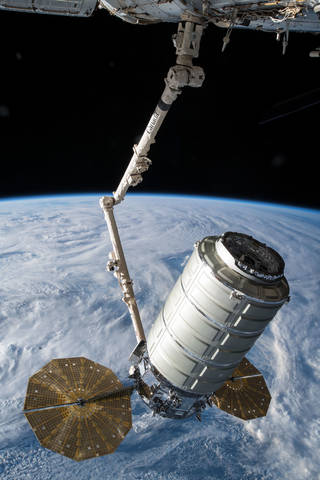
\includegraphics[width=0.25\textwidth]{imagenes/canadarm2.jpg}
    \caption{\cite{81}}
    \label{fig:canadarm}
\end{figure}

Sin embargo, en la mayoría de los casos de uso complejos, la información que estos reciben a través de los receptores no es suficiente para cumplir de manera adecuada con las tareas asignadas, ya que existen restricciones que suponen barreras infranqueables para completar ciertas labores, sean impuestas por el entorno o por la naturaleza de la propia actividad a desempeñar. Es por ello que se sigue esta línea de investigación, para hacer la experiencia del usuario que controla telemáticamente sea más inmersiva y similar a la presencia en el espacio de trabajo. 


\section{Tecnologías inmersivas}
Podemos describir la percepción de nuestro entorno como el producto de la capacidad de nuestra mente para interpretar y poner orden a la ingente cantidad de información que recibe a través de los sentidos. La forma en que se transforman los estímulos recibidos como distintas manifestaciones de reacciones químicas y eléctricas a través del sistema nervioso, y cómo nuestro cerebro ordena ese caos para darle un sentido racional es asombrosa.

Con el brutal aumento en la potencia de cómputo en los últimos años y gracias a la gran apuesta que se ha hecho por las nuevas tecnologías, los resultados conseguidos para la simulación de escenarios ficticios son, en algunos casos, prácticamente indistinguibles de la realidad. Es por ello, que el uso de la realidad virtual, por ejemplo, para recrear parajes, experiencias y sensaciones está cada vez más extendido y ve su auge en nuestros días.

Podemos definir las tecnologías inmersivas, de forma genérica, como la aplicación de los tipos existentes dentro de esta disciplina (VR, AR y MR), usados en conjunción con otros métodos con capacidades multisensoriales, para la intensificación de la experiencia que se trata de simular, como haremos con la retroalimentación háptica \cite{91}. En consecuencia, es ostensible el potencial de esta modalidad para su aplicación en áreas como el desarrollo industrial, la educación, el diseño, etc.

Consecuentemente, consideramos que esta tecnología posee un alto valor para su integración en el marco de trabajo establecido para nuestro proyecto. Así pues, la coordinación de los métodos de teleoperación, junto a la información percibida por el operador del entorno del dispositivo controlado, gracias a los métodos de inmersión, pueden hacer que la experiencia sea satisfactoriamente cercana a la actuación presencial.

\section{Marco de trabajo: IFMIF-DONES}

La evolución del ser humano como sociedad y el consumo de energía en su desarrollo han estado profundamente ligados en el curso de la historia. Tanto es así que incluso fueron propuestos métodos tales como la escala de kardashov, por el astrofísico ruso Nikolái Kardashov \cite{92}, para medir la evolución tecnológica de una civilización en relación a la cantidad de recursos energéticos que esta es capaz de aprovechar de su entorno.

Dicho esto, y congruentemente con lo comentado, es evidente que la dirección en la que se dirige nuestro progreso como sociedad está estrechamente relacionado de forma directa con la forma en que obtenemos y hacemos uso de la energía, y es por ello que se trata en todo momento de encontrar formas efectivas y eficientes tanto de emplearla como de obtenerla, intentando mejorar los procedimientos existentes. 

Actualmente, las principales fuentes de energía utilizadas en todo el mundo derivan de los combustibles fósiles, figura \ref{fig:energy_graph}, energías que no son renovables y cuyas reservas serán agotadas en las décadas venideras. De igual modo, este tipo de comburentes emiten grandes cantidades de gases de efecto invernadero al ser consumidos, y este factor, sumado al cambio climático, cuyos efectos ya son palpables en todo el globo, constituyen una combinación fatal.

\begin{figure}[hbt]
    \centering
    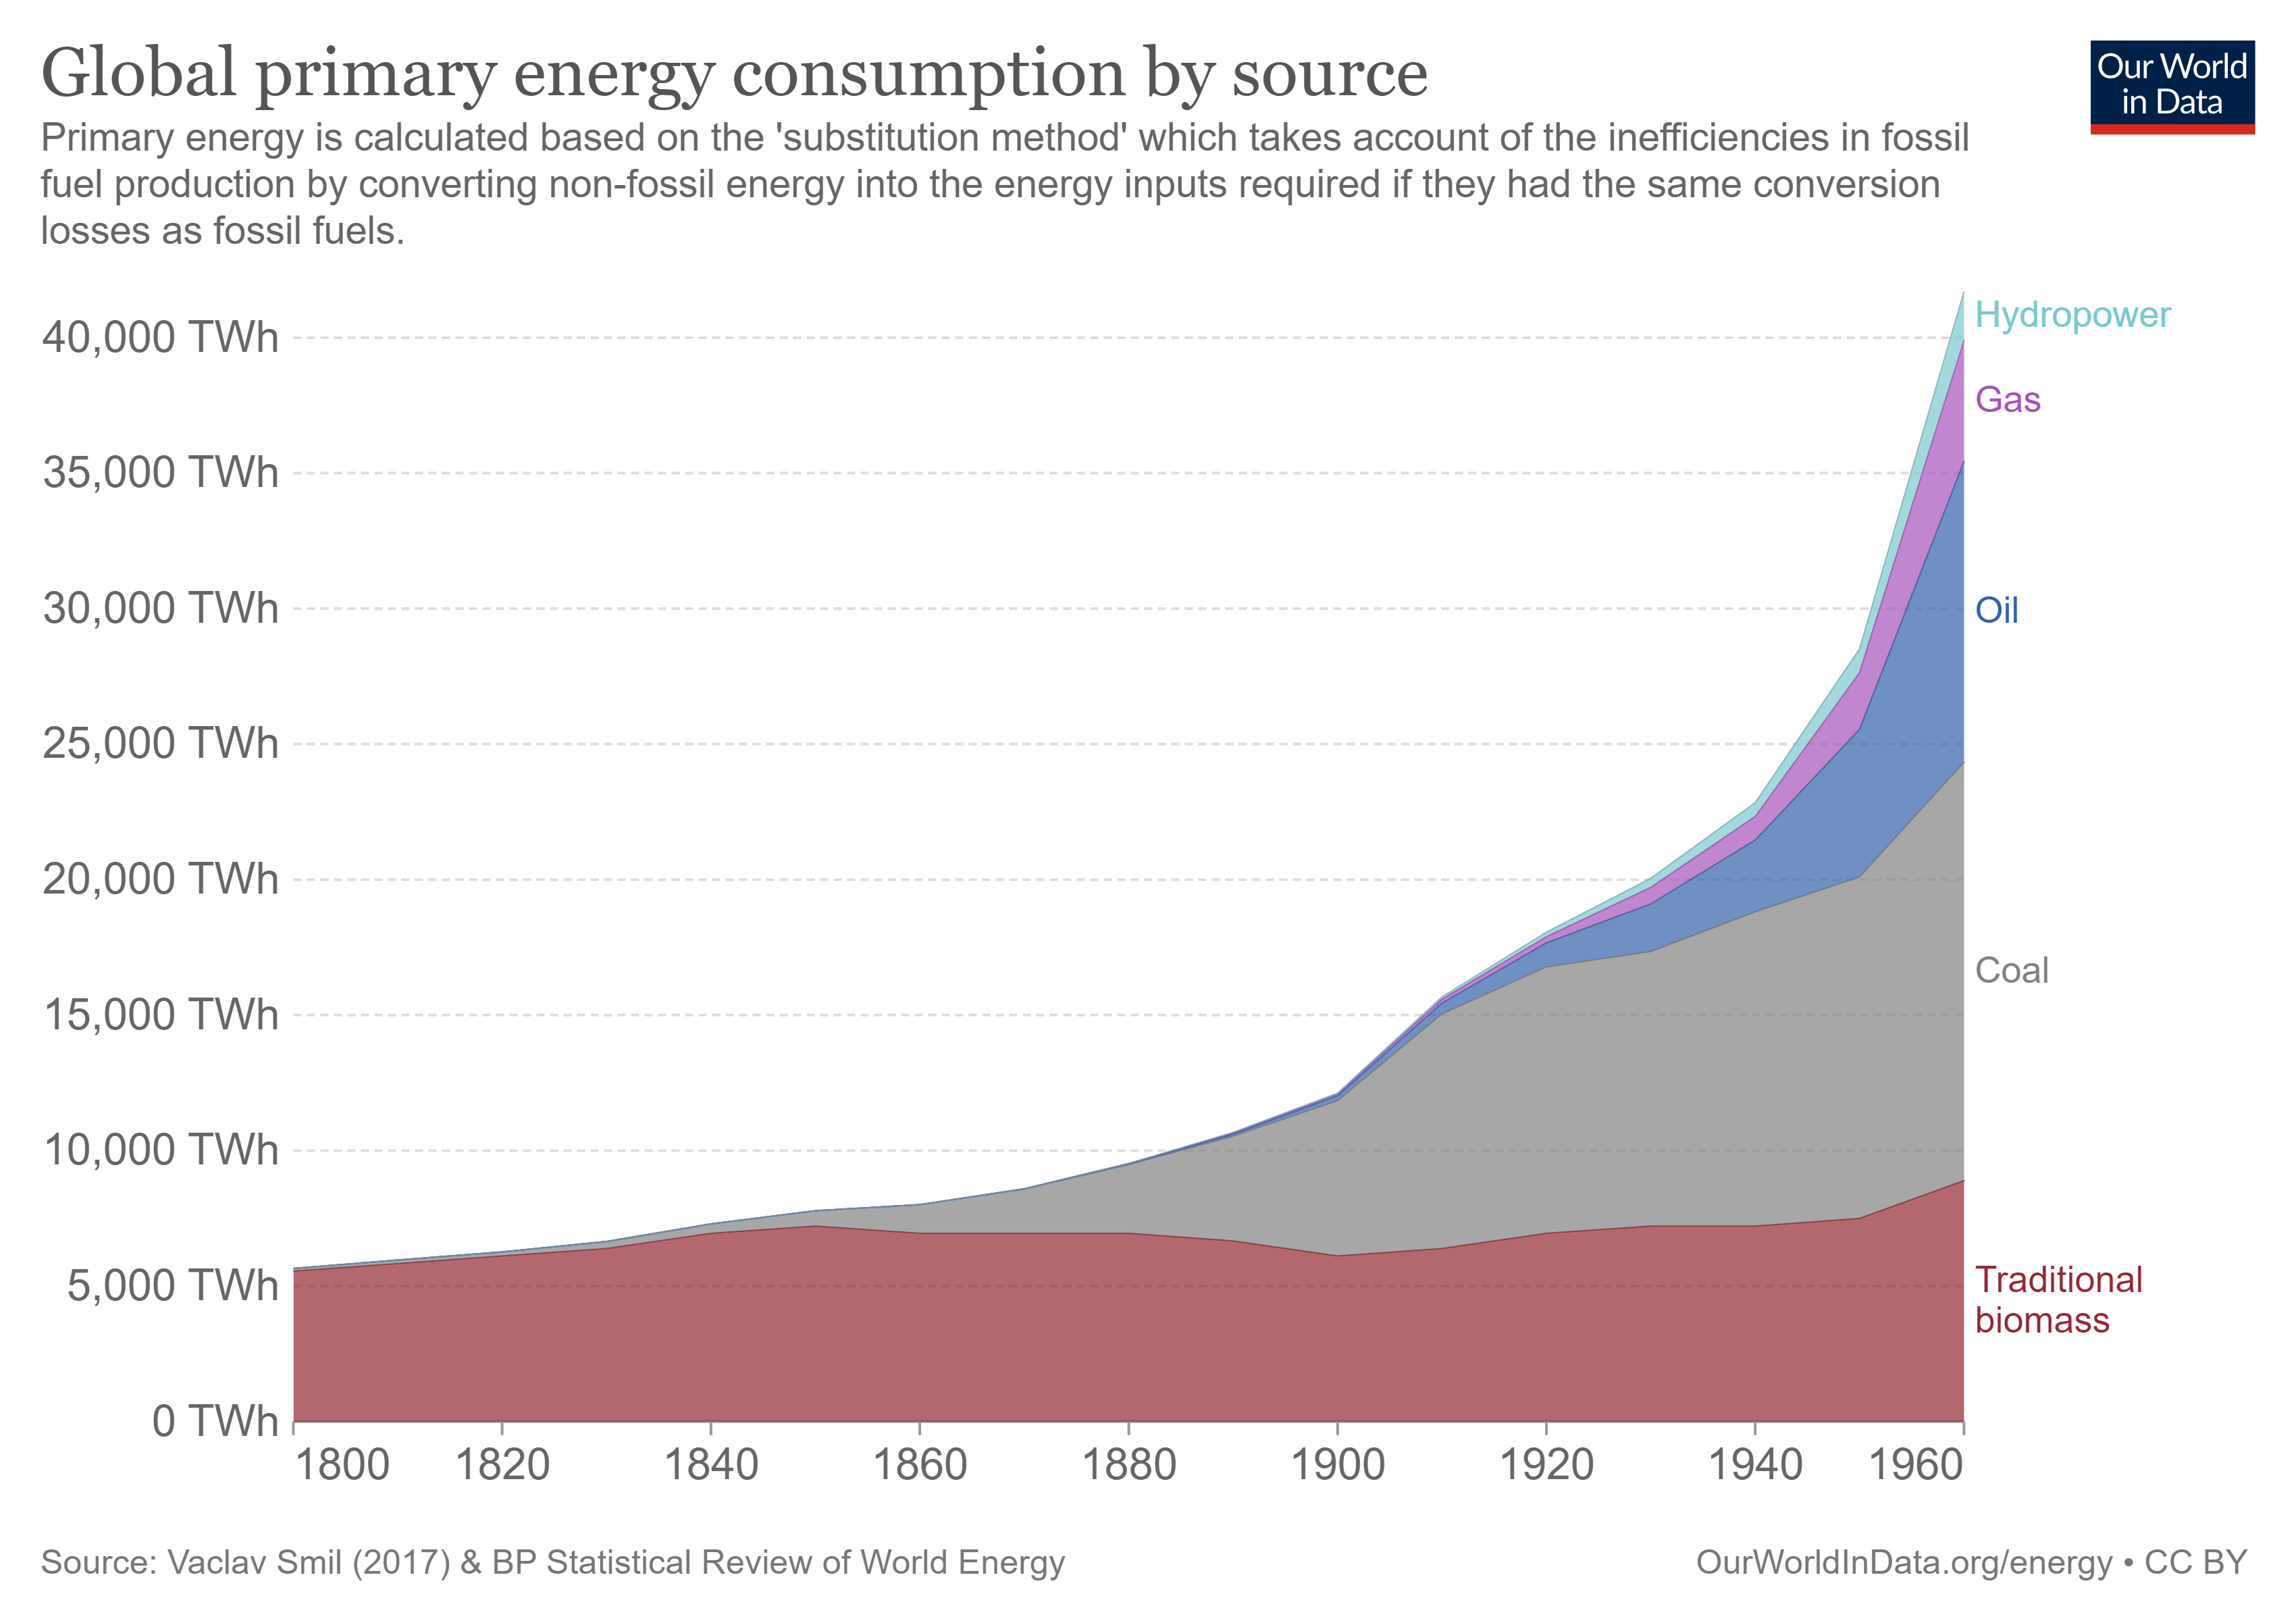
\includegraphics[width=0.75\textwidth]{imagenes/global-energy-substitution.png}
    \caption{\cite{82}}
    \label{fig:energy_graph}
\end{figure}


A ese respecto, se apuesta de forma unánime en todas las naciones por las energías de carácter renovable y con bajas o nulas emisiones para mitigar o reducir los citados efectos del calentamiento global, y es entre ellas que encontramos el motivo de realización de este y otros muchos proyectos que contribuyen a la búsqueda de la obtención de energía a través de la Fusión Nuclear . 

Descrito el contexto que engloba a este estudio, el trabajo de investigación realizado tratará de realizar una aportación en el seno del programa IFMIF-DONES, que figura en la hoja de ruta para alcanzar reactores comerciales que puedan lograr las mencionadas reacciones nucleares.

En este caso, nos centraremos en el apoyo a las tareas de mantenimiento que tendrán lugar; que deberán realizarse en gran parte de los casos a distancia, al menos en las inmediaciones del reactor. Las razones de ello, como cabe esperar, son principalmente las grandes corrientes de radiación que circulan en algunas zonas de las instalaciones, por los isótopos radiactivos de los materiales utilizados en el proceso de fusión y la gran cantidad de neutrones rápidos que se desprenden de las propias reacciones, haciendo de este un ambiente extremadamente nocivo para el ser humano.

\section{Objetivos Planteados}
Los objetivos, como metas que pretenden alcanzarse, definen en esencia las acciones básicas que se realizarán en el marco de un proyecto para, en efecto, trazar una hoja de ruta. En nuestro caso podemos asumir el objetivo general y su motivación como  aclarados en las secciones precedentes.

Como objetivos específicos definiremos algunas tareas que son de obligada consecución para la completa cobertura de los requerimientos que suponemos como básicos y necesarios.

\begin{itemize}
    \item Simular de forma correcta el robot Baxter en Unity para poder trabajar con el mismo en la simulación llevada a cabo. 
    \item Conseguir conectar el dispositivo háptico con Unity y acto seguido tratar de realizar una correspondencia entre ambos robots para lograr el control de Baxter a través del dispositivo háptico.
    \item Tratar de hacer uso de las extensiones existentes para el control del feedback háptico, y en caso de no ser viable investigar la documentación disponible para el artefacto para desarrollar una implementación propia del mismo.
    \item Refinada la reacción al contacto con objetos implementar la posibilidad de agarrarlos y desarrollar la respectiva sensación táctil asociada.
    \item Realizar test de las funcionalidades implementadas para revisar su correcto funcionamiento y rendimiento además de tomar datos acerca del progreso conseguido para realizar gráficas e informes.
    \item Trasladar las posiciones calculadas en las que debe situarse el robot controlado al Baxter real y testear su correcto funcionamiento.
\end{itemize}

\section{Planificación del Proyecto}
El proceso de toma de decisiones previo a la realización de un proyecto, teniendo en cuenta parámetros como el tiempo disponible, los recursos a nuestro alcance y los posibles contratiempos, es una práctica obligada en la correcta ejecución de las tareas que conciernen al campo de la ingeniería y en general a la ciencia. Es por ello que se exponen en esta sección las distintas etapas que se planificaron y por las que ha discurrido nuestro proyecto.

En el diagrama realizado, figura \ref{fig:diagrama_gantt}, podemos observar una progresión clara por distintas fases hasta completar la puesta en marcha y documentación de este proyecto. En principio, podemos asociar a cada una de las semanas de trabajo una media de 30 horas semanales, con lo que la realización completa de este TFG ha tomado alrededor de 330 horas. La idea de planificación inicial se fundamentó en la realización de una nueva tarea cada semana, lo cual se ha intentado respetar al máximo en la medida de lo posible.


\begin{figure}[hbt]
    \centering
    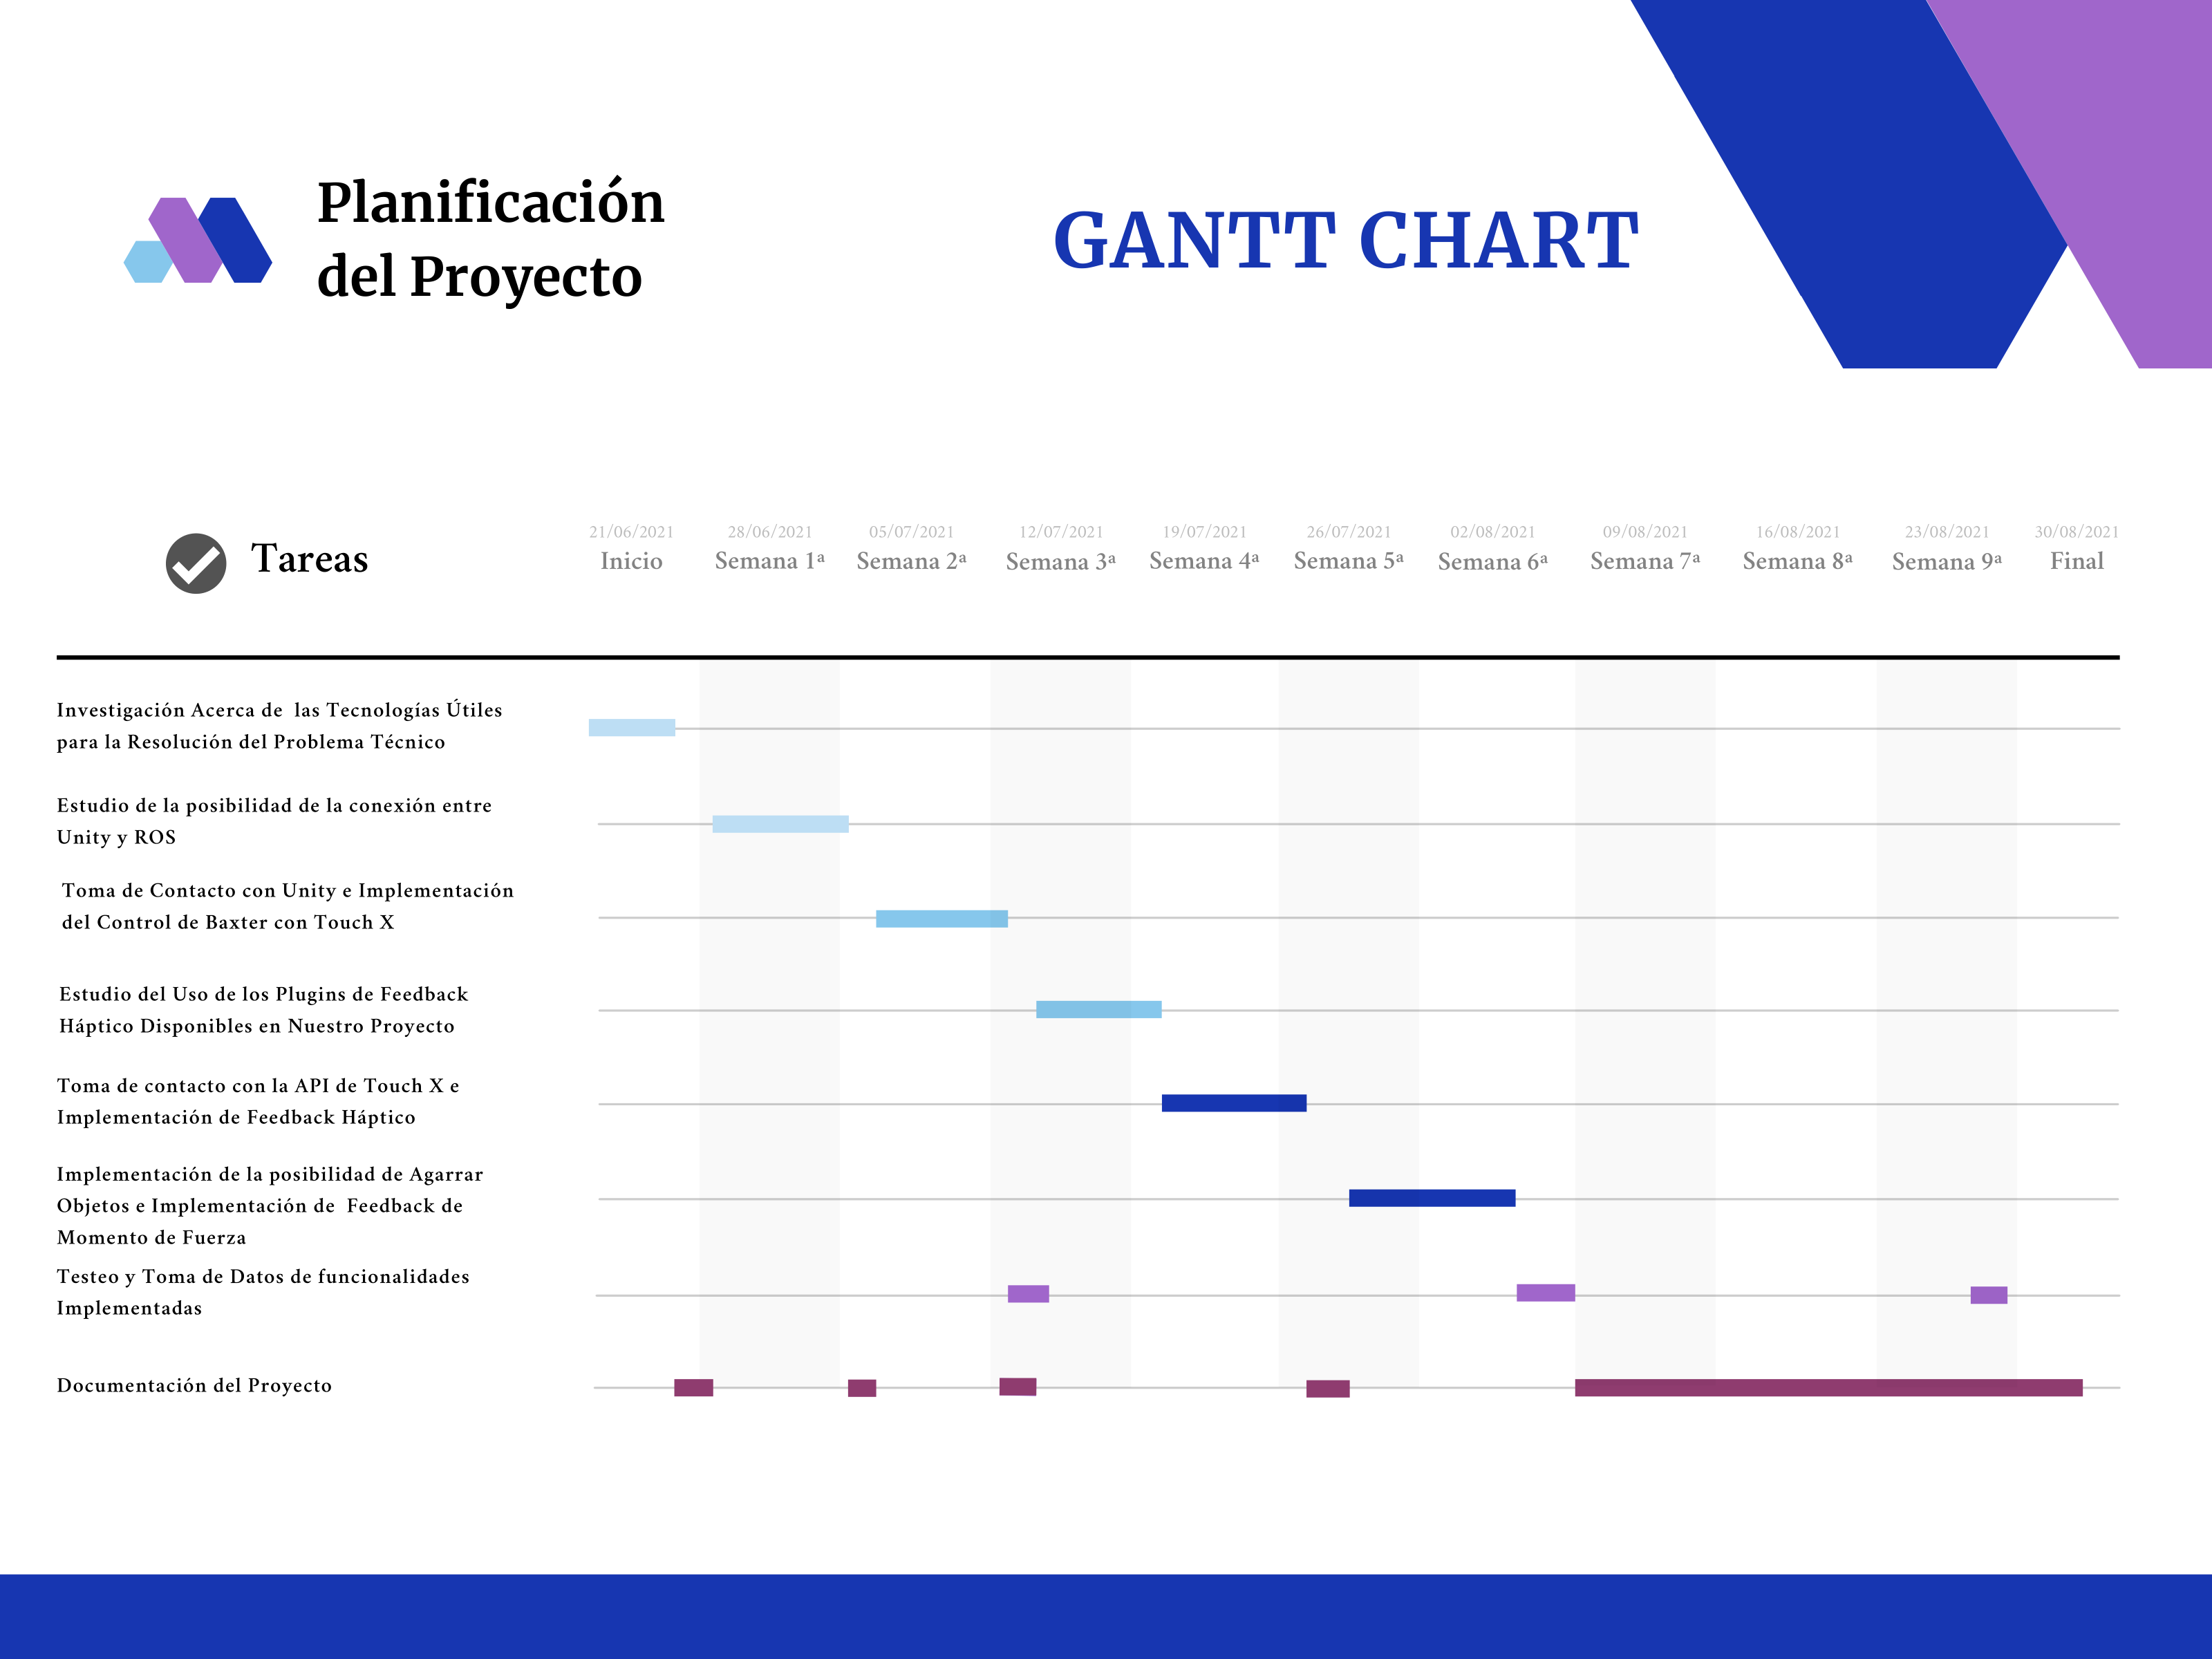
\includegraphics[width=1\textwidth]{imagenes/DiagramaGantt.png}
    \caption{}
    \label{fig:diagrama_gantt}
\end{figure}

En primera instancia, se realizaron tareas de búsqueda acerca de las tecnologías disponibles para la realización del proyecto y el análisis de ventajas e inconvenientes de cada una de las opciones posibles. A tal efecto, la combinación de las tecnologías elegidas resulta  bastante sinérgica, haciendo que la integración de las unas con las otras sea sencilla y eficiente. Adicionalmente, los compañeros en el grupo de investigación en el que este proyecto tuvo cabida trabajan actualmente con algunas de ellas, resultando más sencilla, en caso de ser útil, la integración de la investigación realizada con el resto del proyecto. 

Tras ello, tratamos de realizar la conexión entre Baxter y Unity, explorado así las distintas vías para la consecución de este objetivo, como las extensiones disponibles de las que podíamos hacer uso. Sin embargo, en el momento en que hubimos recabado toda la información necesaria para comenzar la programación, decidimos redistribuir el tiempo, tratando de dedicar una mayor cantidad de horas al feedback háptico y su implementación. Esta decisión se tomó en base a que esta era una característica crucial, considerando pues como opcional esta comentada actividad, ya que la simulación resulta suficiente para nuestra investigación.


A continuación procedimos a tomar contacto con Unity, su entorno y el scripting en C\#. Esta tarea no supuso un impedimento, ya que es conocida la programación orientada a objetos por nuestra parte y se ha trabajado  en ocasiones anteriores con lenguajes derivados de C, con lo que se comenzó con la implementación del control de Baxter en la simulación a través del dispositivo háptico realizando una correspondencia de las articulaciones en ambos robots.

Tras ello, se trató de comprender el funcionamiento de los plugins que materializan el feedback háptico en consecuencia a la simulación para usarlos junto a la parte ya diseñada, pero el resultado fue infructuoso. Se invirtió alrededor de una semana en tratar de llevar a efecto esta solución, ya que resultaba bastante prometedora, pero el uso de los complementos diseñados junto al control implementado por nuestra parte fue imposible. 

En vista a los resultados, se procedió al estudio de la documentación disponible por parte del dispositivo háptico para desarrollar una serie de funciones y scripts que, haciendo uso de la API, gestionan y controlan todo lo que respecta a la monitorización y el manejo del susodicho robot. Esta etapa resultó complicada, y ha sufrido modificaciones hasta el último momento, ya que la decisión final de implementación ha sido fruto del testeo de los distintos métodos existentes para realizar tareas concretas.

Conocida la interfaz de acceso a la máquina, se prosiguió con la simulación de los efectos de gravedad y momento o torque; dos características esenciales para que la sensación táctil se torne lo más fiel a la realidad posible. Para ello se hizo uso de física básica, calculando las medidas de velocidad, aceleración, masa y torque a través de los datos proporcionados por Unity.

Finalmente, en lo que a la toma de medidas y realización de test respecta, podemos ver como en el diagrama se refleja la dedicación de parte del tiempo disponible al final de cada etapa de desarrollo de nuevas características para ello. Tras su puesta en marcha, cada una de las funcionalidades debía ser testeada y ajustada para que el resultado esperado además de ser objetivo resulte agradable y natural para el usuario final.

\section{Estimación de Costos}

La gestión y estimación de costes constituyen una actividad esencial para asignar y controlar exactamente a qué partes se destina el presupuesto disponible para un proyecto. Ello permite a las entidades involucradas conocer de antemano 	la distribución del capital utilizable en el mismo y anticiparse a los gastos que puedan surgir como imprevistos.

Procederemos pues, a realizar un análisis de los equipos y servicios utilizados y a realizar el cálculo de un coste estimado \ref{tab:estimacion_de_costos}.

\bigskip
\bigskip
\bigskip
\bigskip
\bigskip
\bigskip
\bigskip
\bigskip
\bigskip
\bigskip

\begin{table}[hbt]
    \centering
    \begin{tabular}{l p{0.3\linewidth} c c}
        \specialrule{.1em}{.05em}{.05em} 
        \textbf{Servicio} & \textbf{Uso} & \textbf{Unidad} & \textbf{Coste} \\
        \specialrule{.1em}{.05em}{.05em}
        Computador & Realización de tareas de renderizado y simulación & 1 & 277.77 \euro \\
        Dispositivo Háptico & Necesario para el control de Baxter y para proporcionar el feedback háptico & 1 & 8440.00 \euro \\
        Investigador & - & 1 & 554.60 \euro \\
        Licencia de Unity & Entorno de simulación y realidad virtual & 1 & 508.50 \euro \\
        \specialrule{.1em}{.05em}{.05em}
    \end{tabular}
    \caption{Análisis de costos}
    \label{tab:estimacion_de_costos}
\end{table}

El cálculo del coste del computador ha sido llevado a cabo considerando un coste del equipo de 2500\euro  y un uso del mismo en un periodo de 4 meses. De este modo, estimando una amortización de 3 años, el coste valorado es de 277,77\euro.

Para el sueldo del investigador se tiene en cuenta un salario base de 2500\euro, a lo que hay que sumar un 33\% por los costes asociados a la seguridad social en un contrato de 1800 horas anuales. En este caso estimamos unas 300 horas de trabajo, que son las supuestamente destinadas al trabajo de final de grado, con lo que tasamos un importe de 554.60\euro.

En el caso de la licencia para el uso de Unity consideramos que el plan utilizado sería el de Unity Pro, con un coste total anual aproximado de 1,525.51\euro. Sabiendo esto, y considerando un uso por 4 meses, estimamos un importe a pagar de 508.50\euro.

%
\chapter{Estado del Arte}
El estudio del estado del arte, alude en nuestro contexto al trabajo de examinar  y establecer las bases teóricas sobre las que se sustenta la presente obra. En este capítulo detallamos la fundamentación de las ideas en que nos apoyamos y los conceptos clave del ámbito estudiado, necesarios para la comprensión por parte del lector de esta memoria. Junto a ello, se realizará un examen del estado actual de las metodologías implicadas en esta investigación, junto a algunas reseñas históricas relevantes en las disciplinas citadas.

En primer lugar entraremos en materia con la robótica junto a la teleoperación, ya que estas dos especialidades se encuentran bastante ligadas. En este entorno analizaremos sus componentes, las distintas técnicas disponibles, además de su evolución y estado actual para más adelante conocer la razón de su aplicación en este ejercicio.

Sucesivamente, comentaremos las técnicas de inmersión que se usan actualmente y cómo estas han crecido, además de las distintas aplicaciones que tienen y la forma en que pueden aprovecharse para la asistencia en tareas como las desempeñadas en el marco de trabajo establecido.

Finalmente, repararemos en el tema que engloba a nuestro estudio: IFMIF-DONES, conociendo de manera más precisa y profunda el funcionamiento de las instalaciones que se construirán y la relevancia de su fundación para la comunidad científica, concretando así no solo las particularidades que caracterizan las instalaciones de esta índole, sino las de esta específicamente. Junto a ello, pondremos de manifiesto el propósito de la misma y los avances que acarreará en diversos campos de la ciencia además de especificar el lugar que ocupa esta investigación en el marco de este proyecto. 

\vfill

\section{Teleoperación y Robótica}
Trataremos en esta primera sección una de las partes fundamentales para la realización de este proyecto, la robótica. Este interdisciplinario campo de estudio anexa y se nutre del  conocimiento de distintas ramas, como la ingeniería mecánica, eléctrica, informática o la mecatrónica, entre otras. Esta área trata el desarrollo de máquinas que, como se referenció en la introducción, nos permitan llevar a cabo tareas que son imposibles de realizar por personas o que pueden implicar riesgo para seres humanos en su desarrollo.

El propósito de estos artefactos ha variado con el paso del tiempo. En un principio, se pensaron como dispositivos estáticos que realizarían tareas repetitivas y con un grado de complejidad bajo, como lo fue en la industria automovilística \cite{1}.  Sin embargo, en la actualidad, el abanico de tareas que un autómata puede realizar es considerable y continúa en aumento gracias a la investigación. La precisión, rapidez y eficiencia en muchas de las tareas realizadas sumada a la eliminación de los posibles errores humanos, hace de estas máquinas la clave para algunos procesos industriales que poseen un alto grado de automatización.

Por otra parte, y opuestamente a lo que en los inicios de la robótica se consideraba, los robots son designados en la actualidad, además, para gran cantidad de tareas con un alto grado de complejidad que entrañan una considerable capacidad de  de adaptabilidad al entorno, como las desarrolladas por los robots rover de exploración planetaria.


\begin{figure}[hbt]
    \centering
    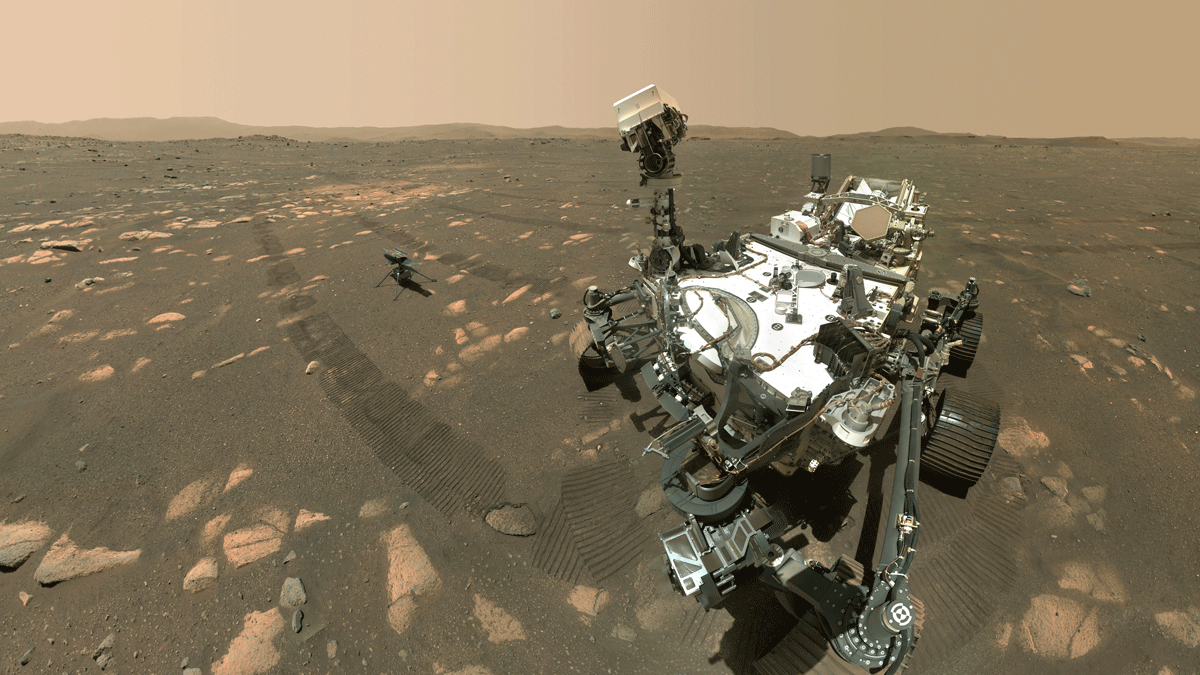
\includegraphics[width=0.5\textwidth]{imagenes/Perseverance.jpg}
    \caption{\cite{83}}
    \label{fig:perseverance}
\end{figure}

Con un peso de 1025 Kg en su lanzamiento y dimensiones similares a las de un automóvil, este dispositivo cuyo diseño está inspirado en el rover Curiosity recorre Marte en su tarea de exploración del cráter Jezero, como parte del desarrollo de una misión de la NASA. La construcción de Perseverance, el robot ilustrado en la figura \ref{fig:perseverance}, es robusta y apta para condiciones de presión y temperatura extremas \cite{2}. Asimismo, es capaz de soportar altas velocidades y aceleraciones, además del impacto de la radiación cósmica, lo hace una máquina versátil e idónea para la tarea para la que está designado.

A pesar de ello, los robots diseñados aún no poseen la capacidad de improvisación y solvencia ante problemas complejos dependientes de una gran cantidad de factores a tener en cuenta en un ambiente dinámico y hostil, como el que en esta investigación nos ocupa. En estos casos, se recurre a la presencia de  operadores para combinar la efectividad y virtudes de ambas metodologías de trabajo. De este modo, es posible omitir el riesgo implícito en el desarrollo de determinadas tareas e introducir la supervisión y control de un manipulador humano.

\subsection{Evolución del Arte}

Con el paso de los años, se ha tratado de forma continua de mejorar las metodologías utilizadas en el desarrollo de distintos procedimientos específicos para su consecución de manera óptima y en el menor período de tiempo posible, logrando así un ahorro en recursos que permite dirigir los esfuerzos disponibles en otros frentes de investigación y trabajo.

La telerrobótica, como parte de este proceso de optimización en el desempeño de ciertas actividades, es un área de la propia robótica que alude al control de máquinas a distancia haciendo uso de otras tecnologías disponibles, normalmente de carácter inalámbrico, como pueden ser Wi-Fi o Bluetooth \cite{3}. De este modo, con el uso de estas herramientas en el desarrollo de ciertas actividades, se consigue la manipulación de elementos de carácter sensible de manera segura y eficaz manteniendo al manipulador del dispositivo en un ambiente protegido.

La teleoperación, estrechamente ligada a la telerrobótica, marca sus orígenes en la industria nuclear. Encontramos un primer ejemplo de esta estrategia de trabajo en el año 1949, cuando Raymond C. Goertz, mientras trabajaba en la AEC, ideó un sistema master-slave cuyo objetivo sería manejar los productos radiactivos resultantes de la fisión nuclear. Tras este exitoso hito, el uso de los manipuladores de acoplamiento eléctrico y su potencial fueron reconocidos, sentándose así las bases de la telerrobótica moderna \cite{4}.

Más tarde, en la década de los sesenta, se trató de extrapolar los estudios realizados al campo de investigación del mar y del espacio, lo que planteó nuevos y desconocidos retos. En esta época se produjeron distintas mejoras, como el uso de cámaras y pequeños dispositivos para aumentar la telepresencia del manipulador. Pese a ello, los sistemas desarrollados denotaban deficiencias en la latencia de control, ocasionando inestabilidad \cite{5}.

Más adelante, a finales de la mencionada década, Victor Scheinman haría muestra de su brazo Stanford, un robot articulado con seis ejes. La máquina desarrollada, tenía la capacidad de seguir con precisión trayectorias señaladas en el espacio, bajo el control de una computadora \cite{6}. 

Tras los comentados inicios, y de forma continua, se producirían relevantes avances en los años sucesivos dentro de esta disciplina, rama de la robótica. Se detallan en la lista siguiente algunos de los avances más significativos, para no prolongar innecesariamente esta contextualización histórica \cite{7}:

\begin{itemize}
    \item 1971 - Formación de JIRA.
    \item 1972 - Creación del brazo del MIT.
    \item 1973 - Presentado robot  T³ con control por computadora por  Cincinnati Milacron.
    \item 1983 - Fundación de Adept Technology.
    \item 1987 - Fundación de la asociación de robótica y automatización del IEEE.
    \item 1988 - Primera Conferencia Internacional sobre Robots y Sistemas Inteligentes en Tokyo, Japón.
\end{itemize}

Observamos tras ello, como esta especialidad cobró relevancia en el panorama tecnológico global y cómo ha crecido con el paso de los años hasta nuestros días, extendiéndose en distintos ámbitos. 

\subsection{Implementaciones Actuales}
Indagando en las implementaciones actuales, se observa que el esquema básico de operación no ha sufrido una  gran cantidad de cambios. Sin embargo, las aplicaciones que implementan esta estrategia de trabajo han aumentado de manera considerable. Pese a que, se señala en gran cantidad de artículos y reseñas a la industria nuclear como principal consumidor y promotor de esta metodología de trabajo \cite{8}, podemos distinguir infinidad de aplicaciones en la actualidad, ya sean militares, industriales e incluso como complemento en distintos campos de estudio, como lo son la biología o la medicina.

\subsubsection{Aplicaciones Militares}
 A lo largo de la historia, gran cantidad de conflictos se han sucedido, siendo esta una  clara manifestación del alto nivel de sofisticación y complejidad de la gestión humana y sus avances tecnológicos. Este dominio, que permite una ingente cantidad de posibilidades, ha sido históricamente una fuente de grandes avances en distintas áreas de la ciencia, entre ellas, la telerrobótica.  

Previamente, cabe destacar que gran parte de las tecnologías de teleoperación se desarrollaron con el fin de apoyar actividades de carácter militar, y figuran entre ellas los dispositivos UAV -comúnmente conocidos como drones- y UGV -como SARGE creado por Sandia National Laboratories-, como los más conocidos. 

Entre las tareas de estos dispositivos figuran la vigilancia, la detección de enemigos, el reconocimiento del terreno, el aseguramiento de bombas, la vigilancia y el apoyo en asaltos entre otros. Tareas que, de algún modo, podrían resultar tediosas o arriesgadas para un ser humano de forma presencial \cite{9}.

\subsubsection{Aplicaciones Espaciales}
Como ya hemos comentado, algunas labores en el espacio requieren del uso de telerrobótica, como las antedichas aplicaciones; aunque las tareas que implican más riesgo para seres humanos y que a su vez nos proporcionan más información, son las de exploración. Desafortunadamente, para tareas de esta índole es prácticamente inevitable el uso de la teleoperación aún. Es por ello que las aportaciones en esta materia han sido mayúsculas por parte de este sector.

Se considera como el primer vehículo teleoperado en la superficie lunar a Lunakhod 1, en los inicios de los años 70. La tarea desempeñada por este dispositivo fue recorrer en torno a 10 kilómetros en los 11 días de duración de la misión. Como se detalló en la reseña histórica, en este tiempo los retardos en los canales de comunicación eran considerables, dificultando la misión. Sin embargo, el sistema Sojourner de la NASA, que sufrió  tiempos de retraso mucho mayores, fue teleoperado con éxito durante 7 días marcianos \cite{10}.

Las razones para el uso de la teleoperación, atisbamos, se tornan bastante claras en este contexto. Entre ellas pueden destacarse: la peligrosidad de las acciones de despegue y aterrizaje, la eliminación de los problemas de latencia, la reducción de costos -ya que los equipos de soporte vital para los astronautas son distintos de los sistemas en el espacio probados en ISS-, los problemas de radiación en superficies planetarias -puesto que son altamente perjudiciales y su mitigación puede resultar costosa- además de que las condiciones en planetas como Venus, Mercurio, Io o Titan son impracticables para nuestra anatomía, debido a las condiciones de calor y presión \cite{11}.

\subsubsection{Aplicaciones Médicas}
La telemedicina, concepto emergido en la década de los 70, surge como un método contra la lucha de las barreras geográficas, aumentando la disponibilidad de los cuidados referentes a la salud singularmente en zonas rurales y países en desarrollo. Como su nombre indica, esta disciplina de la medicina trata de prestar servicios de tratamiento o diagnóstico de enfermedades de forma remota \cite{12}. 

Podemos encontrar distintas noticias en la red acerca de los recientes avances en este campo y sus frutos. En este caso, una de las noticias que más encajan en el ámbito de esta investigación, es la prueba de que ya es posible realizar cirugías u operaciones a distancia, aunque no es la primera vez que esto se practica. 

En este caso, el cirujano Kais Assadullah Rona, demostraba cómo se puede realizar cirugía a 8,000 km de distancia haciendo uso de la red 5G, que presume de tener latencias prácticamente imperceptibles. En las imágenes, podemos ver como el operador corta la piel de una banana, para acto seguido extirpar una pequeña parte y finalmente coser el área con absoluta precisión. Con este hecho, queda patente que tareas de esta índole pueden completarse con éxito sin mayor complicación \cite{13}.
   
\subsubsection{Aplicaciones Submarinas}
Las tareas a llevar a cabo en entornos submarinos, a determinada profundidad, pueden conllevar unos altos niveles  de riesgo para el operario y un alto coste asociado. Como detallamos, el uso de autómatas en este campo también hace acto de presencia, en el mantenimiento de plataformas petrolíferas o en la industria del gas, por ejemplo. 

Para las tareas descritas, y un compendio de las mismas aún más extendido, es usual el uso de ROVs o vehículos submarinos operados a distancia. Este tipo de dispositivos son altamente maniobrables y usualmente son controlados por un equipo que opera a bordo de alguna embarcación en las proximidades o en tierra en las mismas condiciones, ya que la comunicación es cableada. Para el manejo de los brazos manipuladores se usan bombas hidráulicas, que alimentan los sistemas de torsión además \cite{14}.

En adición a lo especificado, se añaden sensores, cámaras y luces para que la experiencia del usuario manipulador sea satisfactoria, teniendo toda la información necesaria.

\subsection{Componentes del Sistema Teleoperado}

La división entre los distintos elementos que componen un sistema teleoperado no es unánimemente aceptada, ya que en algunos casos se suprimen algunas de las partes en favor de su unión con otras. En nuestro caso, tomando como referencia los artículos consultados, consideramos los principales componentes de este sistema como los descritos a continuación \cite{15}. 

\subsubsection{Operador}

Definimos como operador o manipulador a la persona que se encarga del control de las operaciones realizadas a distancia. El control que este ejerce sobre el dispositivo a teleoperar puede ser total y continuo -teniendo así la completa responsabilidad de las acciones del robot en todo momento- o alterno -ejerciendo meramente tareas de monitoreo, planificación o marcado de nuevos objetivos-.


\subsubsection{Dispositivo Controlado} 

Consideramos esta parte como la extensión del operario que trabaja en el lado de control del artefacto teleoperado. El dispositivo controlado, podrá resultar ser un robot, vehículo o sistema que trabajará en la zona remota y responderá a las órdenes de control comandadas por su manipulador.

\subsubsection{Interfaz}

Las interfaces para la teleoperación, y en general en el campo de la informática, poseen un papel de gran relevancia debido a ser las mediadoras entre el hombre y la máquina. Con este término, hacemos referencia tanto a los instrumentos que hacen posible que se efectúe el control del operador, como a cualquiera de los dispositivos que contribuyen en la retroalimentación de este. Encontramos en este punto, una clasificación en distintas categorías: las interfaces directas, multimodales o multisensoriales y de control supervisado.

\subsubsection{Control y Canales para la Comunicación}

Determinamos este componente esencial como el conjunto de medios a través de los cuales se produce el tráfico de información que será enviada y recibida a/desde el dispositivo a controlar. Este módulo será el encargado de la codificación/decodificación de los datos provenientes tanto de los dispositivos para el control como del dispositivo controlado.

\subsubsection{Sensores}

Se denominan como sensores, aquellos dispositivos que se encargan de la recolección de información tanto de la zona remota de trabajo como de la zona local de control para su posterior uso tanto en lo que a interfaces respecta como a lo que al control se refiere.

\section{Técnicas de Inmersión}

Uno de los principales modos de realimentación del entorno del ser humano es la visión. Esta capacidad que poseemos, nos permite distinguir los detalles de nuestro entorno a través de la interpretación, por parte de la corteza visual, de los rayos de luz que inciden en nuestra retina. Podríamos describir pues, la misma, como una de las principales capacidades sensoriales de los homínidos y muchos otros seres vivos.

A ese respecto, aparecen soluciones innovadoras que, ayudadas de la computación, estimulan los susodichos receptores para la consecución de una experiencia visual de contenido simulado tridimensional en tiempo real. Con ello, surgen distintos métodos dentro de este avance tecnológico con objetivos distintos y que se especifican a continuación :
\begin{itemize}
    \item Realidad virtual (VR): esta metodología de emulación del mundo percibido puede describirse como un entorno en el que se recrean escenarios y elementos con apariencia real, generados por tecnologías de carácter informático. Se hace uso, en este caso, de hardware  específico que permite al usuario la visualización de los componentes descritos en un campo de visión similar o superior al de la vista humana en tres dimensiones. Adicionalmente, la simulación obtenida puede ir acompañada de dispositivos que permitan interactuar con el medio representado, intensificando la experiencia \cite{16}.
    
    \item Realidad aumentada (AR): podemos describir esta tecnología como el compendio de métodos utilizados para la representación de un mundo enriquecido con elementos añadidos al mundo real, haciendo que este contenga información suplementaria de carácter gráfico, háptico o sonoro entre otros. Para el logro de esta experiencia se hace uso de dispositivos de distinta índole, desde smartphones a smart glasses, con la capacidad de mostrar los elementos tangibles al alcance del usuario a la vez que reconocerlos y agregarles elementos virtuales \cite{17}.  
    
    \item Realidad Mixta (MR): se alude con este término al acoplamiento entre  la realidad y la simulación mediante dispositivos electrónicos. Con esta definición, podemos inferir que los términos que describen AR y MR se tornan ambiguos entre sí y es común en la literatura su uso indistintamente.

    El propósito de la realidad mixta se fundamenta en el logro de la combinación entre VR  y AR, extendiendo el mundo tangible a la simulación virtual. Para ello, esta nueva concepción del entorno se cimenta en la creación de un modelo tridimensional de aquello que el usuario percibe como real para su posterior potenciación con contenido adicional relevante \cite{18}.
\end{itemize}

En esta sección comentaremos las distintas técnicas de inmersión disponibles, además de su desarrollo a través de los años hasta la actualidad. De forma preliminar,  estableceremos de forma directa la relación que este concepto guarda con el proyecto realizado no sin antes introducir algunos de los conceptos clave. 

Vinculando así, la presente sección con la que le precede, advertimos en varias ocasiones de que en el control de dispositivos de manera no presencial el operario necesita conocer el estado del entorno en el que el dispositivo controlado se encuentra en todo momento, para poder reaccionar ipso facto a distintas situaciones adversas que pudieran tener lugar. Esta noción, entonces, desemboca en un concepto más específico para nuestro propósito, la telepresencia.

El término telepresencia hace alusión al conjunto de técnicas que permiten que una persona perciba, gracias a los sentidos, la impresión de estar presente en el lugar deseado, creando un marco de trabajo realista para el usuario. Así pues, para lograr con la inmersión una completa experiencia de telepresencia, se hace uso de la interacción en tiempo real, una alta capacidad para la visualización del espacio simulado, acompañado de estímulos auditivos que permiten el posicionamiento y capacidades de realimentación táctil para poder sentir el hecho de colisionar, agarrar o manipular objetos en nuestro caso \cite{19}.

\subsection{Evolución del Arte}

El origen de la realidad virtual no es aceptado de forma unánime, ya que la concreción de su definición no resulta sencilla. Pese a ello, las primeras referencias a la definición moderna de este concepto se deben a la ciencia ficción.
 
Se atribuyen a Morton Leonard Heilig, pionero en este campo, los inicios de esta tecnología como la conocemos hoy día gracias a la creación de Sensorama, en 1962. Este artefacto, precursor de las tecnologías de realidad inmersiva multisensorial, más conocida en la actualidad como multimodal, es considerada una de las primeras implementaciones de la realidad virtual.

El dispositivo desarrollado incluía una pantalla estereoscópica, ventiladores, artefactos capaces de emitir distintos olores, un sistema estéreo de sonido y una silla móvil. Con ello, esta máquina tenía capacidad de simular, según se preparó como ejemplo, un viaje en motocicleta por la ciudad de Nueva York, recreando las distintas sensaciones que implicaría este, estimulando los cinco sentidos \cite{20}.

Más adelante, Ivan Sutherland, con ayuda de sus alumnos, crearía la denominada Espada de Damocles, en 1968. Este sistema, predecesor de las gafas y cascos de realidad virtual de los que hoy se hace uso, trató de utilizarse  en tareas de simulación inmersiva. El sistema desarrollado contaba con un casco -que pendía del techo debido a su peso-, un auricular, un sensor de posición de la cabeza, y distintas unidades de cálculo específicas además de un computador de uso general \cite{21}. 

En los años posteriores, este campo de estudio proporcionó instrumentos con fines médicos, militares y en la industria de la automoción. Tanto es así, que en 1979 Eric Howlett con su diseño de LEEP, se considera que sentaría las bases de los actuales cascos de realidad virtual de hoy en día. Los resultados logrados por este sistema fueron sensacionales, ya que se conseguía una realista sensación de profundidad en el amplio campo de visión en el que la imagen estereoscópica creada se extendía \cite{22}.

Más adelante, el término que designa a la Realidad virtual se popularizó a finales de la década de los ochenta por Jaron Lanier, uno de los precursores en este campo del saber. Este desarrolló algunos dispositivos de realidad virtual, entre ellos Power Glove, uno de los primeros artefactos  con esta tecnología con un precio asequible \cite{23}.

Tras este momento, gracias a los avances logrados en esta tecnología, se hizo notar un aumento en la producción de dispositivos de este tipo para el público, implicando relevantes avances en los años sucesivos dentro de este campo. Comentaremos a continuación algunos de los avances más significativos, para no prolongar innecesariamente esta contextualización histórica, como anteriormente \cite{24}:

\begin{itemize}
    \item 1988 - Cyberspace Proyect, primera implementación de VR en una computadora de bajo costo.
    \item 1990 - Sensei8 Corporation, primeros gráficos en tiempo real con mapeo de texturas.
    \item 1992 - Nicole Stenger, Angels: Primera película inmersiva e interactiva en tiempo real.
\end{itemize}


\subsection{Implementaciones Actuales}
Tratando de revisar las implementaciones actuales y los campos de aplicación para este tipo de tecnología, hallamos que en el mercado actual encuentran un buen lugar en la industria del entretenimiento y los videojuegos. No obstante, es evidente su potencial y diversos campos del saber aprovechan sus ventajas.

\subsubsection{Aplicaciones Militares}
Como indicamos anteriormente, el ámbito militar ha sido y es pionero en el uso de las tecnologías más avanzadas. En este campo de aplicación, la realidad virtual es conocida por sus aplicaciones en simuladores de entrenamiento de soldados o en simuladores de vuelo,  para pilotos inexpertos.

Se definen los simuladores de vuelo, como sistemas que tratan de replicar las condiciones de un ambiente real de trabajo en aeronaves, de la forma más precisa y realista posible. Estos sistemas de entrenamiento se crean utilizando la cabina de un avión, que más tarde será montada en una plataforma hexápoda, lo que permite un movimiento con seis grados de libertad. Estos sistemas tienen en todos los casos un coste elevado, por lo que son inaccesibles al público en general.De este modo, podrían reproducirse situaciones de fallo sin el riesgo que implica, ahorro en gastos de combustible y aeronaves, etc \cite{25}.

Por otro lado, encontramos los simuladores de tiro o simuladores de un completo campo de batalla. Haciendo uso de los mismos, los soldados pueden entrenar sus capacidades de tiro, adaptación al entorno, agrupamiento táctico y consciencia de la zona de guerra. Las ventajas de este sistema son evidentes, ya que pueden no sufrir heridas, probar distintas metodologías y entrenar de forma sucesiva sin el elevado coste asociado que ello implica. Ejemplo de ello podría ser VCTS \cite{26}.

\subsubsection{Aplicaciones Espaciales}
En el propio estudio de la Tierra, encontramos escenarios cuyas condiciones evocan las circunstancias extremas que se dan en destinos de otros mundos. Esta analogía, hace que investigadores de todo el mundo traten de comprender y aplicar las citadas tecnologías de realidad mixta y realidad virtual para la exploración del espacio exterior.

La misión BASALT, con tres distintos despliegues, se centró en tratar de realizar ciencia relevante a los campos de la biología, química y geología en entornos inhóspitos terrestres, emulando los que se darán en Marte en futuras expediciones. Con herramientas de realidad virtual y aumentada, es factible el envío de datos más completos por parte de los exploradores o los dispositivos en el terreno de aplicación para su posterior análisis por equipos de investigación. De este modo, además, los científicos en el centro de soporte podrían explorar y dirigir la misión llevada a cabo en el entorno remoto \cite{27}.

\subsubsection{Aplicaciones Médicas}
Figuran entre los casos de uso de las tecnologías citadas diversos ejemplos para la mejora en distintos procedimientos dentro de la medicina, como los listados a continuación.  

El uso de estas metódicas de trabajo, contribuyen en el campo de la educación y formación médica, especialmente en cirugía. Gracias a ello, el alumno puede realizar distintos procedimientos sobre pacientes virtuales o aprovechando las ventajas de la realidad aumentada, haciendo así la práctica más realista y productiva. 

En adición, existen estudios que ponen de manifiesto que la RV podría ser una herramienta útil para mejorar las habilidades quirúrgicas y reducir los errores de los procedimientos quirúrgicos \cite{28}.

Además de ello, ha sido testado la lidia con el agudo utilizado la realidad virtual como técnica de distracción \cite{29,30}, por consiguiente, hay estudios que proponen un papel de la RV en el manejo del dolor crónico al inducir cambios neurofisiológicos más allá de la simple distracción \cite{29,31,32}.

\subsection{Feedback Háptico}
Cuando reparamos el sentido del tacto, nos referimos a aquel que permite a los distintos tipos de organismos vivos lograr la percepción completa de los objetos que le rodean. En ausencia de éste, sería imposible la detección de propiedades como la temperatura, la textura o la dureza de las entidades de nuestro entorno. Es gracias a los receptores nerviosos que nos envuelven y el complejo sistema que comunica estos estímulos al cerebro, que somos capaces de interpretar este tipo de información de nuestro entorno para reaccionar en consecuencia.

En primer lugar, tras esta breve introducción, y para tener una completa compresión de la orientación del  proyecto; es una tarea obligada definir qué es el feedback háptico del que haremos uso. Podemos determinar la retroalimentación háptica, como la simulación por parte de un dispositivo electrónico de la sensación que nos produce el hecho de tocar o interactuar con un objeto o entidad. Dicho esto, se entiende este concepto como la forma en que un dispositivo se interrelaciona con el ser humano a través del tacto; como ya lo hacen de forma habitual por medio de la vista o el oído \cite{33}.

Esta tecnología es conocida desde largo tiempo, y ya es muy usada entre los dispositivos que usamos en el día a día, como nuestros smartphones, consolas e incluso vehículos; asistiendo en tareas como la conducción o concediéndonos una experiencia más inmersiva.

Encontramos en la actualidad diferentes usos e implementaciones con esta metódica, como lo son las plataformas en movimiento, los guantes o los dispositivos desarrollados por openHaptics de los que haremos uso \cite{34}.

\begin{itemize}
    \item Plataformas en movimiento: este tipo de ingenios de la inmersión tiene su origen en los mencionados sistemas de simulación de vuelo. En ellas, el usuario puede sentir la posición en la que se encuentra el elemento simulado, obteniendo consciencia así de cuál sería el comportamiento del dispositivo controlado en la realidad y sus limitaciones . 
    
    \item Guantes: el uso de estos dispositivos para la intensificación de la experiencia virtual es común en ambientes dinámicos que implican la interacción con objetos. Gracias a los dispositivos neumáticos que estos incorporan, el usuario es capaz de sentir la presencia y características del cuerpo en cuestión. 
\end{itemize}

El uso que se dará a esta tecnología en el seno de nuestro proyecto, tendrá el objetivo de aumentar la precisión en el control del robot que realizará las tareas de mantenimiento de forma remota. Estimamos que este, resulta un componente fundamental para una experiencia satisfactoria en el control remoto de cualquier dispositivo, al igual que la retroalimentación visual o sonora.

\section{Entorno en la Fusión Nuclear}
 
Como detallamos en la sección introductoria, la necesidad de energía es uno de los principales problemas que se tratan de solventar desde tiempos inmemoriales. Motivados por su creciente demanda, y por el cambio en las condiciones climáticas terrestres, se trata a través de la investigación y el estudio, de alcanzar formas limpias y altamente eficientes de sustituir las actuales metodologías de obtención de la misma.

En la búsqueda de procedimientos con estas características nos topamos, entre otros, con la fusión nuclear. Este proceso físico tiene lugar en el interior de las estrellas, como nuestro Sol, liberando una ingente cantidad de energía en el proceso. Tanto es así, que percibimos los efectos de la misma en forma de luz y calor, aún a ~151.47 millones de kilómetros \cite{35}. 


\begin{figure}[hbt]
    \centering
    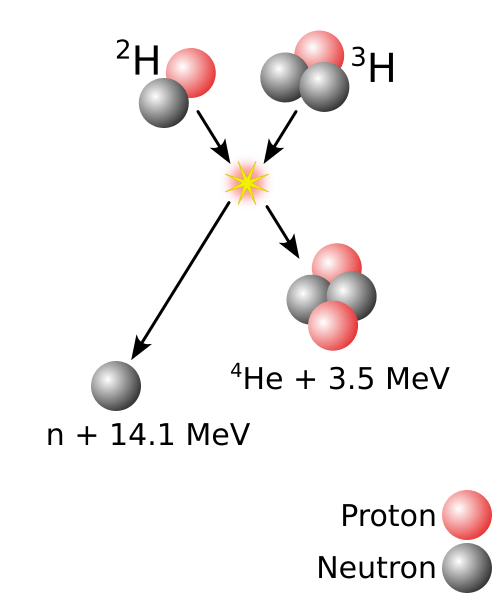
\includegraphics[width=0.3\textwidth]{imagenes/Deuterium-tritium_fusion.png}
    \caption{\cite{84}}
    \label{fig:fusion_reaction}
\end{figure}


Podemos definir la fusión nuclear pues, como el proceso físico por el que varios núcleos atómicos ligeros se unen para conformar un nuevo núcleo más pesado y nucleones, en algunos casos. Sincrónicamente, esta reacción liberará una ingente cantidad de energía -dependiendo de si la masa de los núcleos implicados supera o no la del hierro/níquel-, que permitirá al condensado resultante alcanzar el estado de plasma \cite{36}, figura \ref{fig:fusion_reaction}.

La pérdida de masa que se observa entre los reactivos y los productos, se manifestará finalmente como la energía liberada por la reacción y es explicada a través de la energía de enlace nuclear y el defecto de masa. El primer concepto, hace alusión a la cantidad de energía mínima necesaria para la descomposición de un átomo en sus protones y neutrones, mientras que el segundo, compara la diferencia entre la masa real de un átomo y la masa de sus componentes por separado, que es mayor \cite{37,38}. 

Sintetizando en gran medida, y eludiendo gran cantidad de detalles, es este último concepto es el que explica la citada energía liberada en la fusión, ya que es esta aparente pérdida de masa nuclear la responsable de la misma, como sabemos por la ecuación formulada por Albert Einstein \cite{39}: $$\Delta E=\Delta m * c^2$$.

Son varios los requisitos para conseguir las condiciones que inician y sostienen esta reacción. En primer lugar, es preciso superar la barrera de Coulomb, impulso de repulsión inducido por la fuerza electrostática -que hace que dos protones, por tener misma carga, se repelan- \cite{40}. Para lograr esto, se deben acercar los núcleos atómicos lo suficiente, de modo en que la fuerza nuclear fuerte tenga efecto, ya que en distancias del orden de 1 femtómetro su intensidad es mucho mayor, aunque decae rápidamente hasta ser imperceptible a 2.5 fm \cite{41}. 

Con el objeto de lograr esta reacción en la Tierra, es preciso replicar las condiciones que se dan en estrellas como nuestro Sol, que siguen la reacción en cadena protón-protón \cite{42}. Para ello existen varios métodos y líneas de investigación, pero en nuestro caso especificaremos las características de los reactores de clase “tokamak” de confinamiento magnético \cite{43,44}.

\begin{itemize}
    \item En primer lugar, es necesario el aporte de una ingente cantidad de energía para lograr inducir un primer estado de plasma, -implícito en la constitución de los astros, ya que poseen temperaturas cercanas a los 15 MK- y que puede conseguirse por medio de aceleradores de partículas o láseres.
    
    \item Es de capital importancia lograr un plasma suficientemente denso, para el acercamiento a través de la colisión de los citados núcleos, haciendo que la fuerza nuclear fuerte entre en juego, iniciando el proceso de fusión. (Tercer apartado)
    
    \item Para generar las condiciones de confinamiento -gracias a la gravedad y la compresión en la naturaleza-, se hace uso de campos magnéticos en volúmenes toroidales, para favorecer la estabilidad de los mismos.
\end{itemize}

La fusión es posible con todos los elementos definidos como ligeros -más livianos que el hierro/níquel-, pero la cantidad de este combustible disponible junto al hecho de que la energía a aportar en la fusión Deuterio - Tritio es considerablemente menor -debido a que la citada barrera de coulomb es mucho menor en isótopos de hidrógeno, por contener solo una carga positiva-, hacen de esta la más prometedora, aunque no se abandonan otras combinaciones posibles \cite{45}. 

Este último apartado de nuestro artículo, describe el introducido marco del trabajo realizado, exponiendo los detalles más relevantes para la consecución del objetivo que hemos planteado, además de la problemática y soluciones propuestas, en lo que a la temática de esta obra concierne.


\subsection{Proyectos Asociados}
Para comprender el marco en el que esta investigación tiene lugar, es preciso concretar el propósito de los proyectos asociados a este, cuya conjunción tiene como objetivo final la mencionada fusión nuclear.

\subsubsection{ IFMIF-DONES}
Algunas de las características de los reactores de fusión DEMO aún están por determinar, por razones que se concretan en el apartado dedicado a este proyecto. No obstante, las distintas implementaciones de reactores de este tipo, o posteriormente de fusión comercial, tendrán características comunes; como la presencia de una corriente continua de neutrones desprendidos por la fusión con una intensidad en torno a 14 Mev en el área del primer muro.

En consecuencia, la tarea de caracterización de los distintos materiales que serán utilizados en la construcción de estos dispositivos y la comprensión de cómo se modifica su estructura atómica con el paso del tiempo tras largos periodos de exposición a las antedichas circunstancias se vuelve una labor obligada.

Sin embargo, las condiciones descritas sólo pueden producirse en entornos específicos, ya que las fuentes de radiación disponibles -como lo son la fisión,  la espalación o los haces de iones- no cubren totalmente las necesidades deseadas. Es por ello, que este proyecto tratará de producir un espectro de irradiación de neutrones similar al contemplado en un proceso real de fusión -a través de una fuente basada en la fusión de deuterio y litio acelerada- con suficiente intensidad para el testeo de los materiales de los que se hará uso en las distintas instalaciones DEMO.

Con esta motivación nace IFMIF, la Instalación Internacional de Irradiación de  Materiales de  Fusión, por sus siglas en inglés. El complejo desarrollado, tratará de satisfacer los requerimientos anteriormente descritos con el uso de dos aceleradores lineales de neutrones con 40 MeV de potencia, proporcionando cada uno un haz de 125 mA. Estas fuentes de neutrones acelerados golpearán un chorro de litio líquido produciendo así un intenso flujo de neutrones de cerca de $10^{18}$ N/m²*s (unidad de viscosidad).

Anexo a este proyecto se encuentra DONES, Demo Oriented NEutron Source, cuyo objetivo es el de proveer una fuente de neutrones con suficiente intensidad y volumen de irradiación, como se ha descrito. Además de ello, se tratará de lograr las condiciones de temperatura en las zonas de flujo -250 ºC a 550 ºC-, junto a la acumulación de neutrones que tendrá lugar para producir cedencias de 20-30 (NRT-dpa) en un periodo menor a 2.5 años para 0.3L de volumen y de 50 (NRT-dpa) en lapsos de tiempo inferiores a 3 años, en volúmenes de 0.1L \cite{46}.


\subsubsection{ITER}

ITER,  Reactor Termonuclear Experimental Internacional, es un proyecto en el que colaboran más de 35 países para lograr el mayor experimento de fusión llevado a cabo, aspirando a ser el primer dispositivo de fusión en producir energía neta, es decir, generar más energía de la invertida en el calentamiento del plasma \cite{47}.

De este modo, los objetivos de este dispositivo son claros:

\begin{itemize}
    \item Producir en torno a 500 MW de energía a partir de los 50 MW de potencia inicial necesarios para el inicio de la reacción, aunque no será usado para generar energía en este caso.
    
    \item Poner a prueba los dispositivos, aún en fase experimental, que serán empleados en los futuros reactores, en condiciones semejantes a las que se darán en estos.
    
    \item Conseguir mantener un plasma con reacción deuterio-tritio, capaz de autosostenerse gracias al calor interno generado por la propia reacción, de forma estable y durante un tiempo razonablemente prolongado.
    
    \item Intentar la producción de tritio, a través del denominado “manto fértil”, que se encargará de absorber  gran parte de la energía de los neutrones resultantes de la reacción de fusión, evitando que estos alcancen las bobinas superconductoras y produciendo nuevos neutrones de menor energía que en colisión con moléculas de litio producirán tritio.
    
    \item Evidenciar las condiciones de seguridad de los dispositivos de fusión y sus bajas consecuencias medioambientales.
\end{itemize}

\subsubsection{DEMO} 

Este proyecto, como su propio nombre indica, es el último paso anterior a la fusión comercial. Este tipo de reactor, basado en ITER, deberá ser totalmente operativo a tiempo completo y  tendrá la obligación de demostrar que todas las tecnologías en las que se apoya funcionan con la fiabilidad esperada.

Las especificaciones técnicas relativas a este planteamiento no son tan claras y concisas como en el resto de la hoja de ruta descrita, ya que no hay un consenso de colaboración como en el desarrollo de ITER. No obstante, el diseño presentado por la Unión Europea es conocido y bastante documentado.

Este prototipo está llamado a generar 2 GW de energía continua con el solo uso de 80 MW de entrada térmica inyectada para el inicio de la reacción.  Para conseguir este objetivo, este artefacto deberá tener unas dimensiones un 15\% mayores a ITER y una densidad plasmática un 30\% superior.

Por supuesto, al contrario que ITER, este desarrollo sí contará con la funcionalidad de transformación de la energía liberada -aprovechando el carácter exotérmico de la reacción-, transformando el calor generado en energía eléctrica, para su posterior aporte a la red \cite{49}.

%
\input{capitulos/03_Especificación_de_Servicios_Utilizados}

%
\chapter{Diseño e implementación}
El diseño es el primer paso en la fase de desarrollo de cualquier producto o sistema en el marco de la ingeniería. El objetivo del diseño es la producción de un modelo o representación de una entidad que se construirá posteriormente. [Pressman, 1998]

En este cuarto capítulo de la memoria describiremos los objetivos, respecto a lo a implementación compete, además de las estrategias de programación que seguimos para su consecución. Adicionalmente, aludimos las distintas etapas por las que ha transcurrido el desarrollo y las distintas opciones para el desarrollo de algunas de las funciones que pretendemos llevar a efecto, junto a la justificación de las elegidas. Además de ello, detallaremos la forma de control que se ha tomado en los distintos dispositivos, aclarando algunos conceptos clave, y cómo se ha logrado su funcionamiento a través de las interfaces que el fabricante provee para este fin.

Finalmente, explicaremos de forma breve los fundamentos del concepto físico en torno al que giran la mayoría de las capacidades de realimentación cinestésica que tratamos de proporcionar como información al usuario que utilizará el software desarrollado, el torque. 

Para consultar el código desarrollado puede visitarse el repositorio en github que ha sido utilizado en la implementación de las funciones a continuación detalladas \cite{93}. 

\bigskip
\bigskip
\bigskip
\bigskip
\bigskip
\bigskip
\bigskip
\bigskip


\section{Entorno de Trabajo con Baxter}

\subsection{Inicialización del Entorno}
Antes de poder trabajar con el robot real, como especificamos, se llevará a cabo un estudio para testar la implementación realizada para su control y uso conjunto con el dispositivo háptico. De este modo, describiremos en esta sección algunas de las tareas realizadas como preludio y aclararemos algunos conceptos técnicos relativos que consideramos relevantes.

\subsubsection{Generación de Archivos de Descripción de Baxter}
El primer reto con el que nos encontramos para comenzar con el estudio es la simulación de Baxter en el motor gráfico elegido, Unity. Así pues, en primer lugar, es necesario generar el archivo URDF a través del archivo XACRO que encontramos como descripción de Baxter en el repositorio dedicado al mismo \cite{64}.

\begin{itemize}
    \item URDF: escritos en lenguaje de programación XML, son archivos utilizados en ROS para la descripción completa de robots, tanto en lo que a sus componentes como a sus sensores, enlaces o articulaciones respecta. Es por ello que podríamos modelar cualquier robot a través de este formato e importarlo a ROS para su simulación y análisis \cite{65}.
    
    \item XACRO: por motivos relativos a la extensión de los archivos URDF, es necesario el uso de archivos con un carácter de descripción más genérico y es por ello que se hace uso de XACRO. Este tipo de archivos, que se describen como un lenguaje de macros de XML, permite la construcción de archivos más cortos y legibles usando rutinas que se expandirán a expresiones XML mayores \cite{66}.   
\end{itemize}

Para conseguir generarlo deberemos hacer uso de las herramientas que nos provee  
el propio ROS,  que permiten generar el archivo final a través de las descripciones que provee el archivo XACRO.

\subsubsection{Importación a Unity}
Elaborado el archivo de descripción de Baxter, procederemos a configurar nuestro entorno virtual e incluir el robot. Para modelar los robots simulados, es necesario especificar sus propiedades físicas, mallas de colisiones y mallas visuales \cite{67}.

\begin{itemize}
    \item Mallas Visuales: estas mallas describen la forma, textura y en general el aspecto de los objetos que las implementan de la forma más semejante a la realidad posible.
    
    \item Mallas de Colisiones: este elemento representa el área que ocupa un componente, envolviendo su superficie con la misma. De este modo, Unity es capaz de detectar y calcular la magnitud y el efecto de una colisión entre dos o más componentes, incluidos los propios “enlaces” del robot.
    
    \item Propiedades Físicas: especificamos para cada robot los parámetros que determinan su masa, momento, coeficientes de contacto o dinámica de las articulaciones para su precisa simulación respecto a su comportamiento físico. Con ello Unity podrá efectuar el cálculo del estado del robot respecto a su velocidad, pose o aceleración.
\end{itemize}

En este proceso, gracias a los mencionados archivos URDF, solamente tendremos que incluir los ficheros que describen a Baxter junto al documento URDF que generamos en el árbol de directorios de Unity, preferiblemente en Assets. Acto seguido, haremos uso de una de las extensiones disponibles, URDF Importer, que nos asistirá en este proceso \cite{68}. Una vez importado, solamente deberemos proveer los valores de inicialización del robot en el archivo de configuración asociado para poder usarlo.

\subsubsection{Conexión Entre Unity y ROS}
Una vez Baxter está representado en Unity, será necesario para las pruebas finales en un entorno real la conexión entre este y ROS, para poder enviar los comandos de movimiento al robot real como se describe posteriormente. Para ello, necesitaremos crear una infraestructura de red que soporte la conexión entre ambos. De este modo, necesitaremos que Unity comparta a través de la interfaz de red creada las información relativa  a la posición, velocidad o torque a nuestro middleware, ROS, que a su vez comunicará al robot Baxter la susodicha.


\subsection{Metodología de Control}
Los modos de control que ofrece Baxter son variados, para adaptarse a distintos casos de uso. Para nuestro proyecto se plantearon dos vías de resolución del problema a dirimir: que un teleoperador pueda mover con la mayor libertad posible el robot.


\subsubsection{Cinemática Inversa}
Un primer enfoque para la resolución de este problema, consiste en trazar la punta del dispositivo controlador dentro de un espacio geométrico euclídeo, para conocer el punto objetivo en el que Baxter debería colocar su mano o pinza. Es decir, se debe crear una correspondencia entre el punto señalado por el dispositivo manipulador en la simulación y el entorno real en que actuará Baxter. Para ello, en primer lugar, debería de establecerse una relación lineal entre el radio de acción del brazo de Baxter y del dispositivo háptico para no generar incoherencias. Tras esto, es necesario hacer uso de la cinemática inversa para el correcto movimiento del brazo robótico teleoperado.

Pero antes, es preciso conocer el significado del concepto que designa la nombrada cinemática inversa. En el contexto de la robótica, se designa a esta como la metodología por la cual se realiza el cálculo del movimiento que deberán efectuar las distintas articulaciones componentes de un sistema móvil acoplado para que el efector final se sitúe en la posición especificada \cite{69,70}.

Haciendo uso de esta metodología de trabajo, necesitaríamos realizar el mencionado cálculo en todo momento, para lograr una buena precisión, lo que es realmente costoso computacionalmente. Así pues se plantean para esta alternativa dos caminos posibles: realizar el cálculo de la misma en Unity y enviar los resultados directamente a ROS o enviar la posición final del efector desde Unity y realizar el cómputo de la cinemática inversa para Baxter en ROS. 

\subsubsection{Mapeo de las Articulaciones de Ambos Robots}
Alternativamente, se planteó realizar una correspondencia entre las articulaciones del robot háptico y Baxter. Así pues, aprovechando que el robot háptico cuenta con 6 DOF y Baxter con 7 DOF, podemos hacer concordar el movimiento de las articulaciones una a una preservando el movimiento de uno de los acoplamientos de Baxter en concreto. 

La implementación de esta metodología implica la realización de un mapeo entre cada ángulo del dispositivo háptico con su análogo en Baxter. De este modo, Unity sería el encargado de enviar en todo momento las posiciones de las articulaciones deseadas a ROS para que este las comunique al Baxter real.

Así pues, en primer lugar, seleccionamos las articulaciones del brazo de Baxter según su orden de precedencia en el brazo del mismo, eliminando las que no nos serán útiles. Hecho esto, procederemos a calcular la relación existente entre cada una de las articulaciones seleccionadas y sus homólogas en el dispositivo háptico para establecer una relación lineal entre las mismas, haciendo así que cada desplazamiento en el dispositivo controlador tenga una respuesta proporcional en el dispositivo controlado. Para ello simplemente obtendremos las aperturas de los ángulos de Touch X periódicamente para calcular su correspondencia en Baxter gracias a la correlación dispuesta.

En última instancia, esta es la metodología de implementación que finalmente se ha seguido. El principal motivo de ello es la versatilidad que nos brinda la posibilidad de poder controlar en todo momento la posición de todas y cada una de las articulaciones de Baxter, obteniendo un control más preciso y similar a la interacción del brazo real del operario. Con ello, sabremos en todo momento por dónde pasan los componentes del brazo robótico pudiendo evitar posibles colisiones, ya que la solución que nos ofrece la cinemática inversa no es conocida hasta que se lleva a cabo su cálculo, aunque la solución sea errónea.

\subsection{API Baxter (ROS)}

Como se ha especificado, ROS es el sistema a través del cual establecemos contacto con Baxter. Se define este middleware, como una colección de marcos de software de código abierto para el desarrollo de servicios que incluyen la utilización de robots. Así pues, este proporciona distintas utilidades cuyo diseño está orientado a un clúster de computadores heterogéneo, para el acceso a los recursos hardware. Así pues, se representan los conjuntos de ejecución de procesos en este programa con una arquitectura de grafo, en cual se pueden publicar, recibir o multiplexar los distintos datos que se reciben por parte de los sensores, por ejemplo.

Asimismo, dentro de la reseñada arquitectura, cada uno de los nodos que forman parte del antedicho grafo se conectan a través de enlaces que podemos denominar como tópicos o temas, a través de los cuales se produce el paso de mensajes o llamadas. De este modo, se cuenta en esta estructura con un proceso maestro encargado del registro de nodos y su configuración además de orquestar las comunicaciones entre los mismos. No obstante, una vez creada la infraestructura ésta no actuará como proxy, sino que la comunicación tendrá lugar de nodo a nodo. Para comprender en mayor medida los conceptos introducidos haremos una pequeña descripción de cada uno de los componentes descritos, necesarios para el correcto funcionamiento de una implementación básica \cite{71}.

\begin{itemize}
    \item Temas: Podemos describir este concepto, en el ámbito en que nos encontramos, como un conducto con nombre cuya finalidad es el envío y recepción de mensajes. Estos son creados por el usuario, y su nombre debe ser unívoco en su entorno de alcance para poder publicar mensajes o suscribirse a un tema para recibir de un determinado tipo. Con este modelo de trabajo se preserva el anonimato de los nodos, no conociendo así quién envía los mensajes, sino solamente los propios mensajes. 
    
    \item Nodos: En ROS, un nodo representa un proceso o servicio en ejecución en el contexto de trabajo. Al igual que los temas estos deben poseer un nombre o declararse como anónimos -en cuyo caso se generará un identificador aleatorio para este- y ser registrados con este antes de ejecutar alguna de las acciones programadas en el mismo. En el ciclo de trabajo de este middleware estos son de capital importancia, ya que las acciones que se realizan son producto del procesamiento de datos e información que estos proporcionan y reciben. 

    
    \item Servicios: Este tipo de nodos representan una acción que un nodo podría realizar y que dará como salida un único resultado. Estos son usados a menudo para acciones concretas que seguirán un algoritmo fijo. De este modo, los nodos pueden anunciar servicios y llamar a los mismos entre sí. 
    
    \item Servidor de Parámetros: Podemos describir estos como una base de datos compartida por todos los nodos y que permite el acceso a información que puede resultar útil o necesaria para un conjunto de los mismos. Los datos almacenados en este cambiarán con poca frecuencia, serían pues, buenos ejemplos de ello, las constantes definidas para un robot, como podría ser su rango máximo de amplitud en una de sus articulaciones. 
\end{itemize}

Tras esta introducción a ROS, para comprender de mejor manera la estrategia de trabajo que hemos seguido, se detalla en la figura \ref{Fig:Estructura_Conexion_Unity_ROS} la estructura de conexión entre los distintos procesos que se encargarían de la comunicación entre Unity y Baxter.

\begin{figure}[hbt]
    \centering
    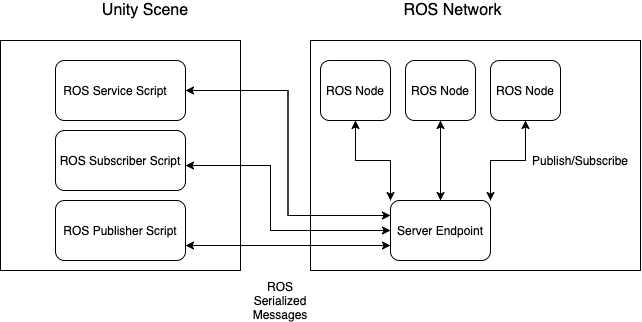
\includegraphics[width=0.75\textwidth]{imagenes/unity_ros.png}
    \caption{\cite{89}}
    \label{Fig:Estructura_Conexion_Unity_ROS}
\end{figure}


\subsubsection{Modo de Control}

Como se especificó, Baxter cuenta con dos brazos -cada uno con 7 grados de libertad- además de poder mover su cabeza en dos ejes. Para poder aprovechar al máximo su movimiento la interfaz de comunicación que posee nos brinda la posibilidad de controlar la posición angular, velocidad y torque de cada una de sus articulaciones para poder situar su efector final en la posición deseada. 

El estado de cada una de las articulaciones puede ser obtenido/establecido mediante mensajes publicados en ROS. Así pues, existen distintos arrays en los que es posible establecer los distintos modos especificados \cite{72}. 

\begin{itemize}
    \item name[i]: id de la i-ésima articulación en los arrays de valores
    \item position[i]: posición de la articulación i-ésima en radianes
    \item velocity[i]: velocidad angular de la articulación i-ésima en rad / s
    \item effort[i]: esfuerzo aplicado en conjunto i-ésima en Nm
\end{itemize}

Los susodichos estados son publicados por robot\_state\_publisher y son actualizados con la información proporcionada por los sensores en cada ciclo. De este modo, la tasa de publicación puede ser establecida mediante la publicación de mensajes de este tópico para lograr una mayor eficiencia o fidelidad.

\section{Entorno de Trabajo con Touch X}

\subsection{Inicialización del Entorno}

Tras inicializar el entorno con Baxter, comenzamos con las pruebas de control del dispositivo háptico y su correcta integración en Unity a través de los plugins y demostraciones disponibles.

\subsubsection{Estudio de la Integración de Touch X y Unity}

Una vez comenzamos la parte del trabajo relativa al control del dispositivo junto a Unity nos topamos con dos principales plugins disponibles en la Asset Store de este último. Los mismos integran funcionalidades y casos de demostración desarrollados en este motor gráfico, haciendo patente que es posible el funcionamiento conjunto de ambas tecnologías.

En primer lugar, procedemos a tratar de conocer su funcionamiento y las llamadas a la API que estos realizan, analizando los scripts que implementan el comportamiento del dispositivo háptico en consecuencia a la simulación. Tras conocer la metodología de trabajo de los mismos, consideramos posible la integración de estos junto a los controladores desarrollados por nuestra parte para el movimiento de Baxter en relación a Touch X.

Entre otras cuestiones, encontramos las mencionadas extensiones están diseñadas para el control de un dispositivo con un volumen y superficie reducidos, extrapolando la aplicación de la fuerza a un solo punto. No obstante esto no es un problema, ya que el feedback que proporcionaremos resulta ser simplemente un vector, por lo que podemos obtener en cada colisión del brazo robótico con los objetos que le rodean todos los puntos de impacto y vectores normales relativos haciendo una sumatoria de las fuerzas resultantes \cite{73,74}.  

Sin embargo, esta metodología de trabajo resulta inviable, ya que el acceso al dispositivo por parte de la susodicha extensión y la metodología de control desarrollada por nuestra parte se torna imposible por errores de exclusión mutua y reserva del dispositivo por parte del primero aparentemente.

Es por ello que decidimos, tras repetidos intentos infructuosos de combinaciones para conseguir lograr la antedicha tarea, desarrollar nuestra propia interpretación de la retroalimentación háptica en consecuencia a la simulación.

\subsection{Metodología de Control}
Asimismo, como se consiguió anteriormente, en primer lugar será necesaria la importación de las funciones implementadas en la citada API, que nos permitirá el acceso a los datos relativos al estado del dispositivo y su control, cuestión que no fue aclarada en la sección que detalla el movimiento de baxter. Para ello haremos uso de los archivos .dll.

\begin{itemize}
    \item DLL: Se denominan bibliotecas de enlace dinámico aquellos archivos compilados cuyo contenido consiste en código ejecutable que se interpreta bajo la demanda de un programa ejecutado en el sistema operativo. 

    Gracias a estos se consigue el empaquetado de información y funciones relativas a un mismo fin reduciendo el espacio necesario para ello, consiguiendo una gran modularización para el acceso por parte de distintas aplicaciones y optimizando la memoria utilizada \cite{75}.
\end{itemize}

Consecuentemente, incluiremos en nuestro proyecto de Unity los archivos del tipo descrito, que se incluyen en el árbol de directorios de instalación de OpenHaptics, para extraer las implementaciones que permiten el acceso a la interfaz de control de Touch X.

\subsubsection{Implementación del Feedback en Colisión}
Como se comentó, en las tareas de mantenimiento que se realizarán en el contexto descrito, será usual la manipulación de objetos. En esta tarea, es relevante conocer la dirección y sentido del impacto que se produce además de la magnitud del mismo para evitar posibles daños a los equipos o las propias instalaciones. Es por ello que la retroalimentación respectiva a los impactos se ha desarrollado de forma en que el usuario pueda sentir levemente los roces o choques leves y que sienta una fuerza bastante más elevada a la hora de tratar de atravesar un objeto.

Detectar que estamos colisionando no es una tarea complicada en Unity, sin embargo, debemos conocer cuál es exactamente la articulación dentro de baxter está colisionando. Para lograr esta tarea haremos que cada una de las articulaciones hijas que componen el brazo notifique su colisión a un script maestro que procesará la información en consecuencia.

Así pues, una vez detectamos el contacto, analizaremos la colisión obteniendo todos los puntos de contacto de la misma para acto seguido calcular el vector de dirección resultante de la suma de todos ellos, obteniendo así la dirección del torque que deberemos establecer en sentido contrario. En este caso, identificaremos si el brazo se encuentra solamente apoyado sobre el plano, estableciendo una fuerza mínima para que pueda sostenerse por sí solo. Además de esto, guardaremos el estado de las articulaciones componentes de Touch X en ese instante para posteriormente conocer cuál es el vector que define la dirección de desplazamiento respecto al instante de colisión.

Asimismo, es una tarea necesaria establecer algunas condiciones para la detección de nuevas colisiones para no confundir los errores de precisión del operario o de las lecturas proporcionadas por Unity y el dispositivo háptico. Es por ello que establecemos distintas consideraciones como no recalcular una nueva colisión si la distancia no supera un cierto umbral establecido a través de sucesivos test en ejecución.

En este momento, como se referenció anteriormente, estableceremos una fuerza de torque creciente dependiendo del desplazamiento que se haga en Touch X, que como sabemos controla a Baxter. De este modo, a través de distintos métodos, determinaremos cuando realmente tratamos de penetrar un objeto y en qué medida pretendemos hacerlo, para establecer una resistencia creciente en el movimiento del dispositivo háptico en esa dirección.

Para ello, establecemos una relación entre los componentes del brazo háptico y el eje al que aportan movimiento, es decir, consideramos el eje de giro de cada articulación para posteriormente realizar una ponderación de la influencia en el desplazamiento en el mismo.

La función elegida para la representación de la fuerza será una exponencial que dependerá de algunas constantes establecidas con el testeo en el proceso de implementación. En concreto definimos una función por partes cuya variable, x, será la cantidad de penetración que se trata de realizar, calculada como la variación entre la posición de las articulaciones al inicio del contacto con un objeto y la actual. Se definen pues $MIN_T = 40$, como el torque mínimo    que utilizaremos y $MAX_T = 1200$, como el máximo a usar.


$$
    f(x)= \left\{ \begin{array}{lcc}
             0 & si  & x < 0.02 \\
            \\ MIN_T + e^{(\ln(MAX_T-MIN_T)/MAX_P)*0.06}*0.7 & si & x > 0.02  \hspace{10pt} y \hspace{10pt} x < 0.06 \\
            \\ MIN_T + e^{(\ln(MAX_T-MIN_T)/MAX_P)*x}*0.7 & si & x > 0.06 \hspace{10pt} y \hspace{10pt} x < 0.1 \\
             \\ MIN_T + e^{(\ln(MAX_T-MIN_T)/MAX_P)*x} & si & x > 0.1\\
             \end{array}
   \right.
$$

Se definen en esta función distintos tramos, establecidos tras la iterativa realización de pruebas. De este modo, la variable $MIN_T$ representará el mínimo torque -establecido como 40 mNm por ser la mínima fuerza necesaria para que el dispositivo pueda sostenerse por sí solo, emulando estar apoyado-. Por el contrario, $MAX_T$ será el valor máximo de torque usado, ya que lo consideramos como suficiente. Así pues, por último, $MAX_P$ se definirá como la máxima penetración establecida para esa articulación, en la cual se alcanza el valor $MAX_T$. En consecuencia, observamos en las figuras \ref{Fig:penetration_02} y \ref{Fig:penetration_03} la evolución del torque para una penetración de 0.2 y 0.3 respectivamente.

\begin{figure}[!htb]
   \begin{minipage}{0.45\textwidth}
     \centering
    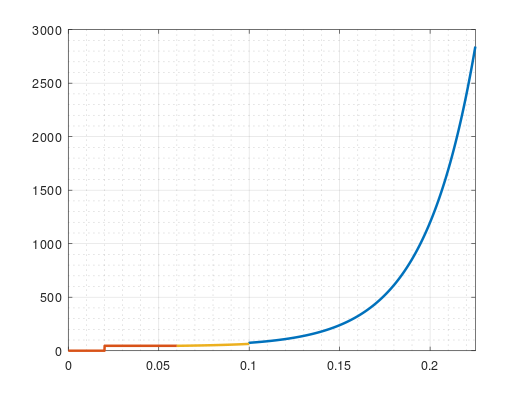
\includegraphics[width=1\textwidth]{imagenes/forceEvolution0.2penetration.png}
    \caption{}
    \label{Fig:penetration_02}
   \end{minipage}\hfill
   \begin{minipage}{0.45\textwidth}
     \centering
    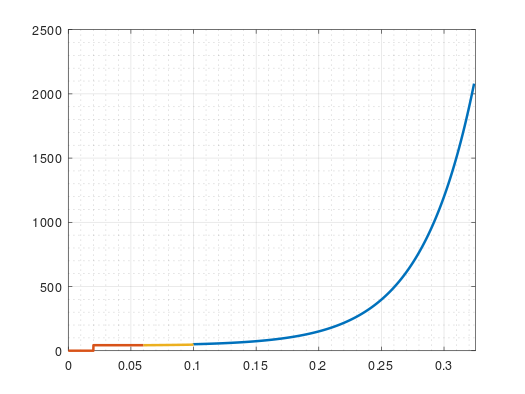
\includegraphics[width=1\textwidth]{imagenes/forceEvolution0.3penetration.png}
    \caption{}
    \label{Fig:penetration_03}
   \end{minipage}
\end{figure}

Gracias a esta y algunos filtros para evitar cambios bruscos, como comparar el nuevo torque que se establecerá con los anteriores valores utilizados, el resultado obtenido se torna agradable al tacto y en general bastante aceptable. 

Además de ello, se toman en consideración algunos casos básicos que se dan en la propia interacción humana con los objetos; como el hecho de solo influir la fuerza normal que nos transmiten los objetos en las articulaciones que preceden a aquella que sufre la colisión,  en el orden que siguen las mismas desde el hombro a la muñeca.

\subsubsection{Implementación de Feedback de Gravedad y Momento de la Fuerza}

Además de conocer las posibles colisiones cuando manipulamos objetos es de gran importancia tener conciencia de la masa asociada a los mismos. En las tareas que conciernen a la teleoperación este factor puede resultar decisivo, ya que a causa de un movimiento brusco o a la carga excesiva de un dispositivo este podría desplomarse. A ese respecto, se ha tratado de realizar una implementación de la gravedad y el torque realistas -contemplando las propiedades físicas exactas de los objetos- a la par que cómoda para el manejo durante un periodo de tiempo moderado.

En este caso, la manera de proceder es bastante intuitiva, ya que consideramos que agarramos un objeto en el momento en que nos acercamos al mismo con el efector final del robot en la simulación y pulsamos el botón que incorpora Touch X en la última de sus articulaciones. No obstante, esta es una mera forma de demostración de las capacidades del dispositivo, ya que Baxter no posee realmente pinzas o manos para prender objetos por defecto en nuestra simulación. Así pues, simplemente sería necesaria la simulación de alguno de los elementos descritos y emular su comportamiento para permitir al robot controlado sujetar elementos de manera realista en la simulación.

Una vez se toma el objeto, se procede al cálculo de las distintas magnitudes intrínsecas en los cuerpos que entran en juego en esta tarea. En este caso utilizamos conceptos básicos de la física newtoniana, como lo son la gravedad, la ley de inercia o la ley fundamental de la dinámica. En consecuencia, cuando el robot agarra un objeto establecemos una fuerza en sentido descendente proporcional al cuerpo prendido, emulando su peso como $\overrightarrow P = m * \overrightarrow g$. En este caso ponderamos las fuerzas entre dos de las articulaciones con feedback en el eje vertical para que la sensación resultante sea una fuerza perpendicular al plano descrito por la superficie en la que se apoya el robot controlado.

Asimismo, procedemos al cálculo del momento de fuerza o torque que sufre el objeto agarrado, despreciando el propio brazo de Baxter para lograr una mayor movilidad y menor cansancio del operario. Por ende, realizamos lecturas en todo momento de la posición del objeto para calcular su velocidad, como $\overrightarrow v =\Delta e/  \Delta t$. Consecuentemente, a partir de la variación de la misma, podemos calcular la aceleración como $ \overrightarrow a = \Delta v/ \Delta t$, para a través del producto escalar de la masa del cuerpo revelar la fuerza en Newtons implícita en el mismo $\overrightarrow F = \Delta a  * m$. Así pues, aplicada la susodicha fuerza a una distancia del punto de aplicación, que será el hombro de Baxter, obtendremos el momento o torque, $\tau = \overrightarrow F*d$ \cite{76}.

Finalmente, como se procedió en la implementación del feedback en el impacto, se establecen distintos métodos para acotar el torque aplicado y evitar movimientos bruscos. Más adelante contemplaremos cómo se lidia con distintos problemas que producen cambios repentinos en el momento aplicado. 

\subsection{API OpenHaptics}
Es necesario hacer uso de su API, como se ha aclarado, para el control del dispositivo háptico. Las interfaces de programación de aplicaciones, se definen como un conjunto de funciones y distintos procedimientos que permiten la conexión y el acceso a los recursos, datos o características de un sistema o aplicación por parte de otro. De este modo, trataremos de controlar Touch X a través de la interfaz que el fabricante nos provee a través de las funciones implementadas en los mencionados archivos .dll que se nos proveen en la instalación del entorno de trabajo del mismo, como se aclaró.

Disponemos de dos maneras de fabricar un nuevo plugin o script controlador haciendo uso de la API que el fabricante del dispositivo nos provee: HDAPI y HLAPI, de las que hablaremos más adelante. La primera obliga al desarrollador a administrar la representación de la fuerza o resistencia que ofrecerá el dispositivo háptico, mientras que HLAPI trata los cálculos de representación háptica basada en primitivas geométricas, transformaciones y propiedades de los materiales proporcionadas por el usuario, lo que resulta en una menor dificultad para el programador; a costa de una ligera pérdida de flexibilidad \cite{77}.

\subsubsection{HDApi}
La interfaz de aplicación HDApi del dispositivo, de la cual hemos hecho uso para la implementación en este estudio, puede ser dividida en dos componentes esenciales principalmente, como lo son el propio dispositivo y el planificador de tareas incorporado. De este modo, la construcción de la interfaz para el acceso al dispositivo permite el soporte de distintos robots con retroalimentación háptica comercializados por 3DSystems.

En este caso, las llamadas a funciones permiten al programador planificar distintas tareas que se ejecutarán en el bucle servidor que se pone a disposición en el momento de uso. De este modo, como se procede en la implementación realizada para este estudio, un programa típico inicializará el dispositivo y el planificador ejecutando a continuación los comandos de realimentación háptica que estime oportunos, para finalmente detener todos los servicios haciendo uso de las llamadas disponible para este fin y cerrar el programa.

Es en la ejecución de los antedichos comandos de realimentación háptica, parte más relevante en el uso del robot, que encontramos algunos aspectos a tener en cuenta en el uso de la interfaz que se nos provee. En primer lugar, será necesario activar explícitamente las capacidades hápticas deseadas a través de las llamadas a la API, entre ellas la realimentación de fuerza. Tras ello, en cada operación de acceso al dispositivo para la consulta o fijación de valores para alguna de sus características será necesario el uso de los denominados como marcos hápticos. De esta manera, los susodichos definen un ámbito o contexto en el cual se garantiza que el estado del dispositivo será consistente y, por ende, todas y cada una de las operaciones que se deseen realizar deberán  ejecutarse dentro de los mismos.

Así pues, cabe destacar que que la programación de las funciones en esta estrategia de control tienen un carácter procedural, de modo que deberemos acceder a los valores, tanto en lectura como en escritura, con el paso de valores por referencia y accediendo a los parámetros deseados a través de códigos hexadecimales definidos en los archivos de implementación \cite{77}.

\subsubsection{HLApi}
HLApi es una interfaz diseñada para facilitar la programación de los dispositivos hápticos soportados basada en patrones de OpenGL para el renderizado gráfico construida en C. Esta permite, como se esbozó anteriormente, la definición de primitivas geométricas, como lo son las líneas, triángulos o puntos junto a propiedades específicas que pueden ir acompañadas de propiedades intrínsecas en los materiales que nos rodean como lo son la rugosidad o una alta fricción. 

De este modo, trabajamos de manera similar a la anteriormente descrita HDApi, teniendo que hacer uso de los comandos disponibles para modificar o consultar las características de los objetos representados. Consecuentemente, el estado de un cuerpo descrito por los algoritmos implementados en el robot incluye información relativa al material del que está hecho, el modo en que se renderiza o las posibles transformaciones que pueda sufrir en su movimiento. Del mismo modo, al igual que en HDApi, es posible consultar el estado de los componentes del dispositivo.

En esta metodología de trabajo, tras el renderizado de las figuras especificadas a la API, es característico el uso del renderizado proxy, que se basa en el uso de un punto que sigue la posición del puntero que describen los efectores finales de dispositivo háptico. Así pues, el citado puntero o proxy se actualizará constantemente pudiendo tocar las figuras representadas en sus caras exteriores, aunque pueden especificarse explícitamente las deseadas. La forma en que el dispositivo tratará de penetrar los modelos y por consiguiente la forma en que se hará la representación de la fuerza, será estirando un resorte virtual entre la posición del dispositivo háptico y la posición del comentado puntero \cite{77}.

\subsection{Torque}
Consideramos necesario en este apartado hacer una breve aclaración acerca de los conceptos físicos implicados en el desarrollo de la implementación que se ha llevado a cabo, para lograr así una mayor comprensión de la totalidad de los conceptos implicados en esta obra. Por consiguiente, expondremos a continuación algunas nociones básicas relativas al campo de la mecánica newtoniana que entran  en juego en la representación virtual de los objetos que nos rodean en lo que a las propiedades táctiles respecta.

La citada teoría mecánica vectorial, formulada por el conocido físico Isaac Newton, se considera una formulación específica de la mecánica clásica en el estudio del desplazamiento de los cuerpos y partículas macroscópicas en un sistema de referencia euclídeo. Por consiguiente, esta da por hecho que se comparte un tiempo por todos los presentes en los eventos de este tipo y asume que los descritos sistemas se desplazan a través de  trayectorias definidas.

De este modo, haciendo uso de las medidas de la variación de la posición, velocidad y aceleración, se designa como momento de una fuerza, o torque respecto a un punto de aplicación, a la magnitud obtenida como el producto vectorial del vector que describe la posición del punto en el que aplicamos la fuerza y aquel que representa la fuerza implícita en el cuerpo. Así pues, congruentemente con este enunciado, podemos representar lo descrito mediante la ecuación dada \cite{78,79}:

$$\overrightarrow M = \overrightarrow {OP} \times \overrightarrow F = \overrightarrow r \times \overrightarrow F$$

Así pues, la interpretación de este concepto en el contexto que describe la aplicación de fuerzas en el contacto con objetos o el desplazamiento de los mismos al ser sujetados por Baxter cobra sentido, ya que esta magnitud física describe la capacidad que una fuerza posee para cambiar la rotación o estado de movimiento del cuerpo al que se aplica la fuerza. De este modo, la fuerza normal que presenta un plano al tratar de realizar un esfuerzo por atravesarlo o la fuerza que un objeto posee en su desplazamiento por el hecho de tener aceleración, teniendo en cuenta el brazo de baxter como punto de aplicación, resulta en el torque que representamos y ofrecemos como retroalimentación al usuario.

%
\chapter{Resultados}
El análisis de los resultados logrados es una de las partes finales obligatorias y conclusivas en la labor de investigación. En esta, procesamos la nueva información surgida como producto de la misma para presentarla de manera ordenada; tratando de conseguir la comprensión del lector y poder ligar los datos obtenidos a unas determinadas conclusiones.

En este capítulo de la memoria, realizaremos un pequeño análisis de las capacidades conseguidas en la implementación realizada para este estudio. Puesto que es complicada una interpretación objetiva de  una sensación tan subjetiva como lo es el tacto, trataremos en esta sección de poner de manifiesto el funcionamiento de la realimentación háptica lograda proporcionando información acerca de la misma. Para ello, realizaremos distintos test y pruebas comprobando así su eficacia y casos límite, exponiendo por medio de gráficas y el análisis de los valores que se toman en su funcionamiento. Así pues, en todo momento, trataremos de desarrollar una interpretación imparcial de los resultados obtenidos en base a los datos recogidos. 


\bigskip
\bigskip
\bigskip
\bigskip
\bigskip
\bigskip
\bigskip
\bigskip
\bigskip
\bigskip
\bigskip

\section{Benchmarks}
Se utiliza esta palabra, proveniente del inglés, para el designio de las comparativas de rendimiento cuyo objeto es el cotejo o testeo de los sistemas aludidos, de modo que nos permitan conocer en qué medida es bueno su funcionamiento o cuál es su grado de rendimiento respecto a unos valores fijados. 

De este modo, trataremos en esta sección de reflejar a través de distintos test el funcionamiento de las dos principales capacidades hápticas implementadas, como lo son la realimentación del momento de fuerza de los objetos prendidos por Baxter o la sensación de colisión con los mismos. 

\subsection{Gráficas de Evolución del Momento}
En primer lugar en este análisis, trataremos la implementación de la gravedad y el torque en el movimiento de un objeto simulado siendo agarrado por nuestro robot controlado. 

Así pues, como se explicó, un objeto posee un momento de fuerza o torque en el momento en que este se desplaza en relación a un punto de referencia con una cierta aceleración. Consecuentemente, extrapolándolo a nuestra propia experiencia, podemos sentir como al tomar un objeto y moverlo deliberadamente este ofrece una cierta resistencia a cambiar su estado de movimiento, sea para iniciarlo o para pararlo, teniendo que ejercer una fuerza en sentido contrario para ello.

Adicionalmente, la por todos conocida gravedad terrestre, impone a todos los cuerpos que caen bajo su acción un constante efecto de caída libre, empujando los mismos hacia su centro de gravedad con una de aceleración constante, mas no uniforme en todos sus puntos. Por ende, cada vez que sujetamos un objeto podemos sentir su peso, como consecuencia de la masa intrínseca en las entidades aludidas.

En el control de Baxter a través de Touch X, para esta sección de la investigación, hemos tratado de establecer un marco de pruebas controlado, en la medida de los posible, para que las mediciones realizadas sean claras y objetivas. Las gráficas que se muestran a continuación son el fruto de la toma de medidas en repetidas ocasiones para obtener valores promedios y representativos del conjunto total. En este caso, describimos la configuración para el testeo como una prueba de carácter real y que podría tener lugar en un escenario en el que nuestro robot realiza tareas de mantenimiento en el comentado ambiente de trabajo en IFMIF-DONES. Asimismo, Baxter tratará de desplazar en repetidas ocasiones un objeto real con 46.13 Kg de masa a través de los ejes X, Y, Z -figuras \ref{Fig:x_axis_baxter}, \ref{Fig:y_axis_baxter}, \ref{Fig:z_axis_baxter}- siendo controlado por un ser humano en todo el proceso. De este modo, aunque este no soporte dicha carga en un entorno real, queda patente la eficacia de la realimentación háptica que podría ser usada en cualquier otro dispositivo solamente modificando los mencionados parámetros de reescalado si fuese necesario.  


\begin{figure}[htb]
    \hfill
    \centering
   \begin{minipage}{0.33\textwidth}
    \centering
    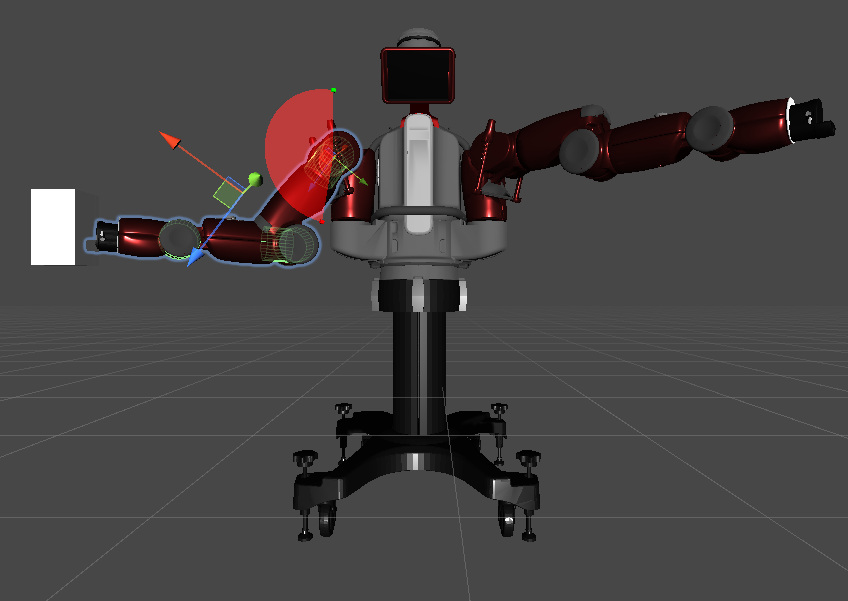
\includegraphics[width=0.9\textwidth]{imagenes/Baxter_Grabbing/FrontViewGrabbing.png}     
    \caption{}\label{Fig:x_axis_baxter}
   \end{minipage}\hfill
   \begin{minipage}{0.33\textwidth}
    \centering
    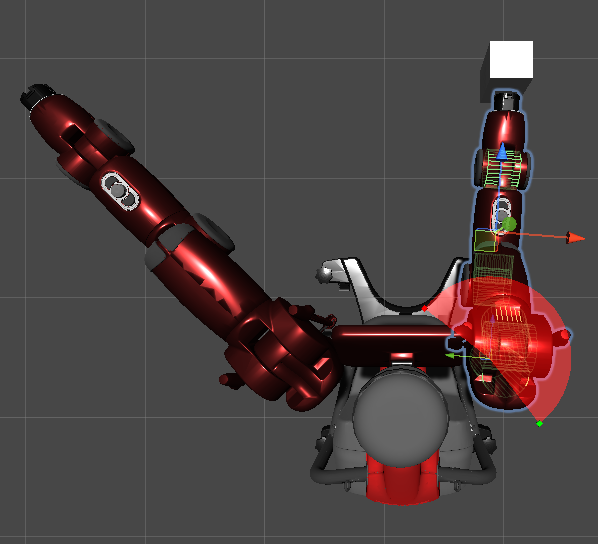
\includegraphics[width=0.8\textwidth]{imagenes/Baxter_Grabbing/TopViewGrabbing.png}     
    \caption{}\label{Fig:y_axis_baxter}
   \end{minipage}\hfill
   \begin{minipage}{0.34\textwidth}
    \centering
    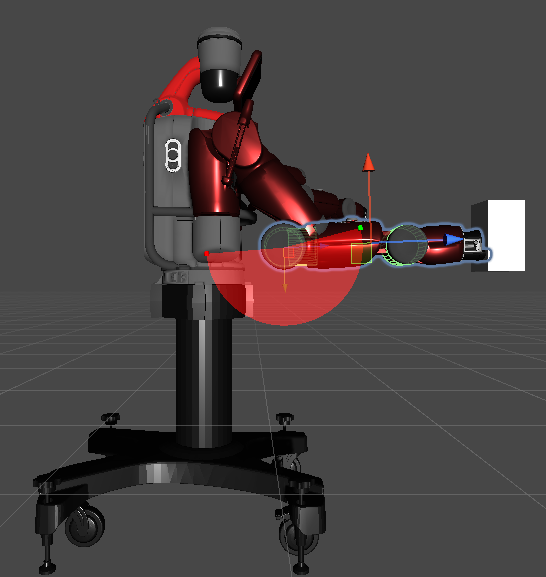
\includegraphics[width=0.7\textwidth]{imagenes/Baxter_Grabbing/LateralViewGrabbing.png}     
    \caption{}\label{Fig:z_axis_baxter}
   \end{minipage}
\end{figure}

Consecuentemente, monitorizaremos los valores establecidos para la simulación del comentado efecto y los representaremos de forma gráfica. En este caso, observaremos en ellas la evolución del torque frente al paso del tiempo en la simulación, medido en ms.

De igual manera, en el proceso de testeo, se lleva a cabo además el reajuste y refinamiento de algunos de los parámetros de reescalado que controlan algunos aspectos decisivos en la simulación de los citados efectos cinestésicos para que resulten lo más agradables al tacto, por lo que especificaremos en todo momento cuales son con exactitud.


\begin{figure}[htb]
   \begin{minipage}{0.33\textwidth}
     \centering
    \includesvg[width=1\textwidth]{imagenes/Mediciones_Torque/Sin_Filtro/Movimiento_en_X_frente_a_Tiempo.svg} 
    \caption{}\label{Fig:no_filter_pentration_test_x}
   \end{minipage}\hfill
   \begin{minipage}{0.33\textwidth}
     \centering
    \includesvg[width=1\textwidth]{imagenes/Mediciones_Torque/Sin_Filtro/Movimiento_en_Y_frente_a_Tiempo.svg} 
    \caption{}\label{Fig:no_filter_pentration_test_y}
   \end{minipage}
   \begin{minipage}{0.33\textwidth}
     \centering
    \includesvg[width=1\textwidth]{imagenes/Mediciones_Torque/Sin_Filtro/Movimiento_en_Z_frente_a_Tiempo.svg}     
    \caption{}\label{Fig:no_filter_pentration_test_z}
   \end{minipage}\hfill
\end{figure}

Los valores de escalado del momento y la gravedad son de 1.0, la ponderación de la misma en los ejes X, Y, Z resulta ser 1.0, 0.0, 0.0 respectivamente. Figuras \ref{Fig:no_filter_pentration_test_x},  \ref{Fig:no_filter_pentration_test_y},  \ref{Fig:no_filter_pentration_test_x}.

En esta primera serie de datos observamos los resultado en una ejecución en la que no establecemos ninguna compensación o comparativa con las fuerzas anteriormente calculadas. Como consecuencia, vemos como el rango en que se mueve la fuerza calculada es muy grande y algunos de los valores calculados muy pequeños, lo que resulta en una mala experiencia final por los golpes con un alto valor de fuerza repentinamente y los efectos de vibración. 

\bigskip
\bigskip
\bigskip
\bigskip
\bigskip


\begin{figure}[!hbt]
   \begin{minipage}{0.33\textwidth}
     \centering
    \includesvg[width=1\textwidth]{imagenes/Mediciones_Torque/Filtradas/Ponderacion_con_1/Movimiento_en_X_Media_ponderada_con_1.svg}     \caption{}\label{Fig:filtro_medias_1_x}
   \end{minipage}\hfill
   \begin{minipage}{0.33\textwidth}
     \centering
    \includesvg[width=1\textwidth]{imagenes/Mediciones_Torque/Filtradas/Ponderacion_con_1/Movimiento_en_Y_Media_ponderada_con_1.svg}     \caption{}\label{Fig:filtro_medias_1_y}
   \end{minipage}
   \begin{minipage}{0.33\textwidth}
     \centering
    \includesvg[width=1\textwidth]{imagenes/Mediciones_Torque/Filtradas/Ponderacion_con_1/Movimiento_en_Z_Media_ponderada_con_1.svg}     \caption{}\label{Fig:filtro_medias_1_z}
   \end{minipage}\hfill
\end{figure}

Los valores de escalado del momento y la gravedad son de 0.3, la ponderación de la misma en los ejes X, Y, Z resulta ser 1.0, 0.0, 0.0 respectivamente. Figuras \ref{Fig:filtro_medias_1_x},  \ref{Fig:filtro_medias_1_y},  \ref{Fig:filtro_medias_1_z}.

Con la sola comparación y promedio del torque actual y el anterior además del escalado en gravedad e inercia la mejora es palpable en la propia gráfica, ya que el rango de fuerzas en el que nos movemos resulta más comprensible por nuestro sentido del tacto. No obstante, aún fallan algunos aspectos como la gravedad, que resulta incómoda o poco precisa.

\begin{figure}[!htb]
   \begin{minipage}{0.33\textwidth}
     \centering
    \includesvg[width=1\textwidth]{imagenes/Mediciones_Torque/Filtradas/Ponderacion_con_2/Movimiento_en_X_Media_ponderada_con_2.svg}     \caption{ }\label{Fig:filtro_medias_2_x}
   \end{minipage}\hfill
   \begin{minipage}{0.33\textwidth}
     \centering
    \includesvg[width=1\textwidth]{imagenes/Mediciones_Torque/Filtradas/Ponderacion_con_2/Movimiento_en_Y_Media_ponderada_con_2.svg}     \caption{ }\label{Fig:filtro_medias_2_y}
   \end{minipage}
   \begin{minipage}{0.33\textwidth}
     \centering
    \includesvg[width=1\textwidth]{imagenes/Mediciones_Torque/Filtradas/Ponderacion_con_2/Movimiento_en_Z_Media_ponderada_con_2.svg}     \caption{ }\label{Fig:filtro_medias_2_z}
   \end{minipage}\hfill
\end{figure}

Los valores de escalado del momento y la gravedad son de 0.2, la ponderación de la misma en los ejes X, Y, Z resulta ser 0.7, 0.0, 0.1 respectivamente. Figuras \ref{Fig:filtro_medias_2_x},  \ref{Fig:filtro_medias_2_y},  \ref{Fig:filtro_medias_2_z}.

En este punto observamos que la gravedad resulta más agradable al tacto, aunque los cambios en el momento de fuerza aún son imprecisos y la ponderación de la gravedad inadecuada. Sin embargo, podemos observar como en cada oscliación en el control a través de Touch X se producen crestas de fuerza, que es el comportamiento esperado. 

\begin{figure}[!htb]
   \begin{minipage}{0.33\textwidth}
     \centering
    \includesvg[width=1\textwidth]{imagenes/Mediciones_Torque/Filtradas/Ponderacion_con_4/Movimiento_en_X_Media_ponderada_con_4.svg}     \caption{ }\label{Fig:filtro_medias_4_x}
   \end{minipage}\hfill
   \begin{minipage}{0.33\textwidth}
     \centering
    \includesvg[width=1\textwidth]{imagenes/Mediciones_Torque/Filtradas/Ponderacion_con_4/Movimiento_en_Y_Media_ponderada_con_4.svg}     \caption{ }\label{Fig:filtro_medias_4_y}
   \end{minipage}
   \begin{minipage}{0.33\textwidth}
     \centering
    \includesvg[width=1\textwidth]{imagenes/Mediciones_Torque/Filtradas/Ponderacion_con_4/Movimiento_en_Z_Media_ponderada_con_4.svg}     \caption{ }\label{Fig:filtro_medias_4_z}
   \end{minipage}\hfill
\end{figure}


\begin{figure}[!htb]
   \begin{minipage}{0.33\textwidth}
     \centering
    \includesvg[width=1\textwidth]{imagenes/Mediciones_Torque/Filtradas/Ponderacion_con_8/Movimiento_en_X_Media_ponderada_con_8.svg}     \caption{ }\label{Fig:filtro_medias_8_x}
   \end{minipage}\hfill
   \begin{minipage}{0.33\textwidth}
     \centering
    \includesvg[width=1\textwidth]{imagenes/Mediciones_Torque/Filtradas/Ponderacion_con_8/Movimiento_en_Y_Media_ponderada_con_8.svg}     \caption{ }\label{Fig:filtro_medias_8_y}
   \end{minipage}
   \begin{minipage}{0.33\textwidth}
     \centering
    \includesvg[width=1\textwidth]{imagenes/Mediciones_Torque/Filtradas/Ponderacion_con_8/Movimiento_en_Z_Media_ponderada_con_8.svg}     \caption{ }\label{Fig:filtro_medias_8_z}
   \end{minipage}\hfill
\end{figure}

Los valores de escalado del momento y la gravedad son de 0.2, la ponderación de la misma en los ejes X, Y, Z resulta ser 0.9, 0.0, 0.1 respectivamente. Figuras \ref{Fig:filtro_medias_4_z},  \ref{Fig:filtro_medias_4_y},  \ref{Fig:filtro_medias_4_z}, \ref{Fig:filtro_medias_8_x},  \ref{Fig:filtro_medias_8_y},  \ref{Fig:filtro_medias_8_z}.

Advertimos que el filtro de medias de orden x respecto al torque escala correctamente, percibiendo mejoras tanto en los gráficos como en la realimentación háptica proporcionada . De este modo, notamos que los resultados obtenidos comienzan a asemejarse a funciones matemáticas concocidas. Además podemos ver como la gravedad se representa el eje X, apreciándose un torque constante y negativo en el mismo.

\begin{figure}[!htb]
   \begin{minipage}{0.33\textwidth}
     \centering
    \includesvg[width=1\textwidth]{imagenes/Mediciones_Torque/Filtradas/Ponderacion_con_10/Movimiento_en_X_Media_ponderada_con_10.svg}     \caption{ }\label{Fig:filtro_medias_10_x}
   \end{minipage}\hfill
   \begin{minipage}{0.33\textwidth}
     \centering
    \includesvg[width=1\textwidth]{imagenes/Mediciones_Torque/Filtradas/Ponderacion_con_10/Movimiento_en_Y_Media_ponderada_con_10.svg}     \caption{ }\label{Fig:filtro_medias_10_y}
   \end{minipage}
   \begin{minipage}{0.33\textwidth}
     \centering
    \includesvg[width=1\textwidth]{imagenes/Mediciones_Torque/Filtradas/Ponderacion_con_10/Movimiento_en_Z_Media_ponderada_con_10.svg}     \caption{ }\label{Fig:filtro_medias_10_z}
   \end{minipage}\hfill
\end{figure}

Los valores de escalado del momento y la gravedad son de 0.2, la ponderación de la misma en los ejes X, Y, Z resulta ser 0.9, 0.0, 0.1 respectivamente. Figuras \ref{Fig:filtro_medias_10_x},  \ref{Fig:filtro_medias_10_y},  \ref{Fig:filtro_medias_10_z}.

Tras la realización de esta ingente cantidad de pruebas notamos que el feedback cinestésico es bastante bueno y se asemeja a la implementación de los complementos desarrollados por parte de 3DSystems, compañía creadora del dispositivo. En este caso podemos ver como la función obtenida toma una forma sinusoidal, debida en cierto modo al balanceo en el testeo.

\bigskip
\bigskip
\bigskip
\bigskip
\bigskip
\bigskip
\bigskip
\bigskip
\bigskip
\bigskip

\begin{figure}[!htb]
   \begin{minipage}{0.33\textwidth}
     \centering
    \includesvg[width=1\textwidth]{imagenes/Mediciones_Torque/Filtradas/Ponderacion_con_12/Movimiento_en_X_Media_ponderada_con_12.svg}     \caption{ }\label{Fig:filtro_medias_12_x}
   \end{minipage}\hfill
   \begin{minipage}{0.33\textwidth}
     \centering
    \includesvg[width=1\textwidth]{imagenes/Mediciones_Torque/Filtradas/Ponderacion_con_12/Movimiento_en_Y_Media_ponderada_con_12.svg}     \caption{ }\label{Fig:filtro_medias_12_y}
   \end{minipage}
   \begin{minipage}{0.33\textwidth}
     \centering
    \includesvg[width=1\textwidth]{imagenes/Mediciones_Torque/Filtradas/Ponderacion_con_12/Movimiento_en_Z_Media_ponderada_con_12.svg}     \caption{ }\label{Fig:filtro_medias_12_z}
   \end{minipage}\hfill
\end{figure}
Los valores de escalado del momento y la gravedad son de 0.2, la ponderación de la misma en los ejes X, Y, Z resulta ser 0.9, 0.0, 0.1 respectivamente. Figuras \ref{Fig:filtro_medias_12_x},  \ref{Fig:filtro_medias_12_y},  \ref{Fig:filtro_medias_12_z}.

Finalmente intuimos que llegamos a un máximo en el escalado de esta técnica. En este caso, la realimentación proporcionada ya no es tan agradable al tacto y resulta confusa en algunos casos. Además de ello los cambios en el sentido de la fuerza resultan excéntricos resultando en pérdidas en los extremos.

Tras las distintas pruebas realizadas decidimos hacer uso de media móvil de orden 10 \cite{80}, lo que favorecerá la estabilidad en el desarrollo de actividades que impliquen su uso y dificultará los cambios bruscos en las mismas. Este valor es elegido tras la valoración de los gráficos expuestos y la sensación en la propia mano en el testeo. En perspectiva este no es un valor muy alto, ya que la función encargada de actualizar los valores del momento o de la gravedad se ejecuta en cada frame, y los frames tienen lugar entre 60 y 80 veces por segundo en nuestro equipo. A ese respecto, una nota importante a considerar es que la potencia del equipo puede afectar en gran medida al renderizado de la retroalimentación háptica, ya que en los casos en que se utilizaba una alta resolución para la visualización de las cámaras en el desarrollo de la prueba podíamos notar cierta cadencia en la misma.

En conclusión, cabe destacar que las pruebas han sido llevado a cabo por un ser humano, lo que hace que tengan un carácter más real. No obstante, al no hacer un manejo totalmente exacto del dispositivo podemos haber introducido, una pequeña cantidad de ruido.

\subsection{Gráficas de Evolución de Torque en Colisión}
Continuando pues con el testeo de las funcionalidades desarrolladas, trataremos en este apartado la evolución del torque que sentiremos en la colisión con los distintos objetos con los que el robot controlado puede interactuar en la simulación o, en una fase más avanzada, en el mundo real.

De este modo, como reseñamos anteriormente, en el momento en que tratamos de realizar una fuerza para tratar de cambiar el estado de reposo de un cuerpo, hace acto de presencia una fuerza normal que interpretamos como una aparente resistencia por parte del mismo en sentido contrario, que en consecuencia a la extensión del brazo de Baxter se manifestará como un torque que deberemos reflejar. 

Consecuentemente, podemos ejemplificar este hecho con un caso cotidiano de uso como es el apretar una simple tuerca haciendo uso de una llave inglesa. En este caso aplicamos una fuerza en su extremo que, a causa de la distancia al punto de referencia -el propio perno-, resultará en un torque aplicado. 

Al igual que en la experimentación y testeo en el apartado anterior, en este caso se trata de establecer un ambiente de pruebas realista a la par que lo más pulcro posible. De este modo, los resultados que presentamos dimanan de los ensayos iterativos y la toma de medidas en promedio de las susodichas pruebas realizadas. Así pues, tomaremos nota de la evolución de la fuerza al tratar de atravesar un objeto simulado como inamovible en los ejes X, Y, Z de la forma que ejemplifican las figuras \ref{Fig:FrontViewCollidingX},  \ref{Fig:FrontViewCollidingY},  \ref{Fig:LateralViewCollidingZ} respectivamente.

\begin{figure}[htb]
	\hfill
	\centering
	\begin{minipage}{0.33\textwidth}
		\centering
		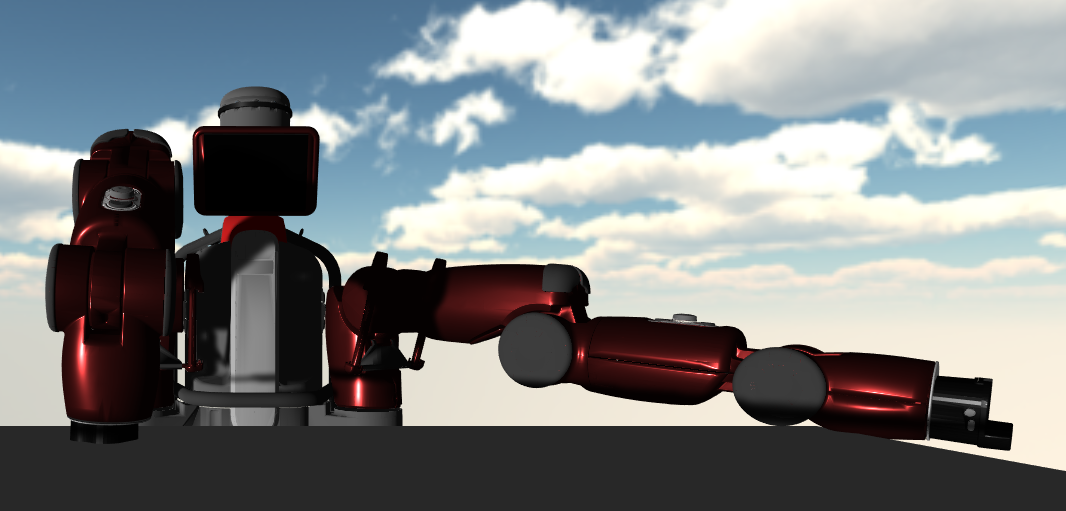
\includegraphics[width=0.8\textwidth]{imagenes/Baxter_Colliding/FrontViewCollidingX.png}     
		\caption{}\label{Fig:FrontViewCollidingX}
	\end{minipage}\hfill
	\begin{minipage}{0.33\textwidth}
		\centering
		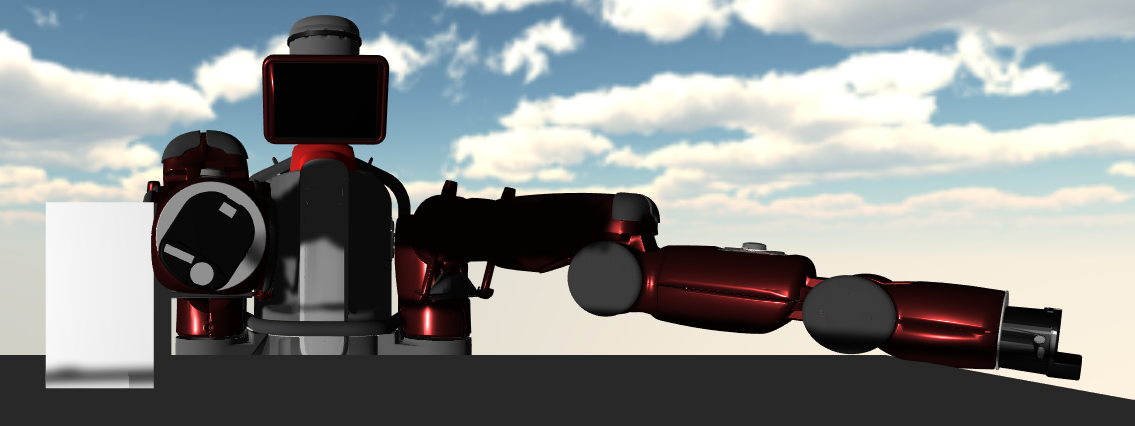
\includegraphics[width=1\textwidth]{imagenes/Baxter_Colliding/FrontViewCollidingY.png}     
		\caption{}\label{Fig:FrontViewCollidingY}
	\end{minipage}\hfill
	\begin{minipage}{0.34\textwidth}
		\centering
		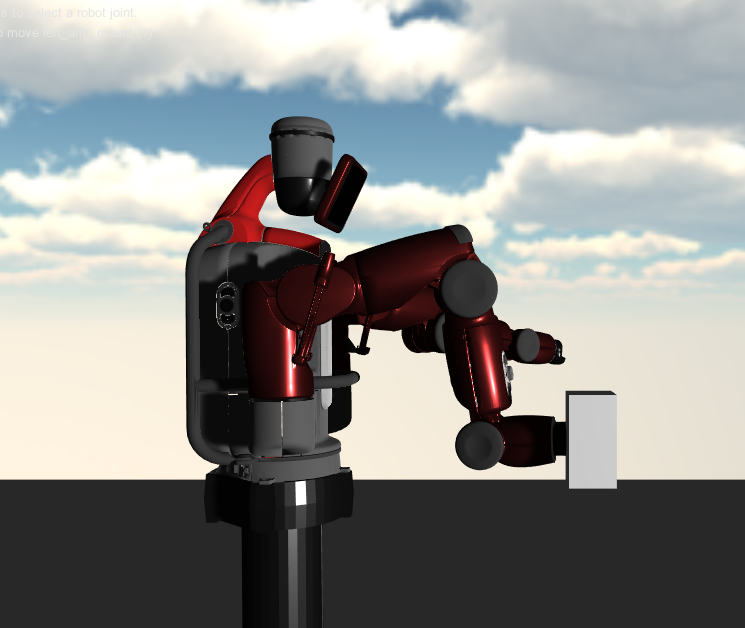
\includegraphics[width=0.6\textwidth]{imagenes/Baxter_Colliding/LateralViewCollidingZ.png}     
		\caption{}\label{Fig:LateralViewCollidingZ}
	\end{minipage}
\end{figure}

La  función que seguirán las intensidades de la realimentación háptica es la ya comentada exponencial, definida en el epígrafe dedicado a la implementación. Asimismo, la función teórica diseñada posee la característica de poder especificar, dependiendo del parámetro divisor del logaritmo, el valor en el que se alcanzará el valor máximo de torque especificado en metros. Por ende, haremos pruebas de ejecución variando este factor representando en este caso los valores de torque -en mNm- que se asocian a distintas intensidades de penetración, que mediremos en cm. 

\begin{figure}[!htb]
	\begin{minipage}{0.33\textwidth}
		\centering
		\includesvg[width=1\textwidth]{imagenes/Medidas_Colision/10/Torque_frente_a_ Penetracion_en_X_Maximo_10.svg}     \caption{ }\label{Fig:penetracion_x_maximo_10}
	\end{minipage}\hfill
	\begin{minipage}{0.33\textwidth}
		\centering
		\includesvg[width=1\textwidth]{imagenes/Medidas_Colision/10/Torque_frente_a_ Penetracion_en_Y_Maximo_10.svg}     \caption{ }\label{Fig:penetracion_y_maximo_10}
	\end{minipage}
	\begin{minipage}{0.33\textwidth}
		\centering
		\includesvg[width=1\textwidth]{imagenes/Medidas_Colision/10/Torque_frente_a_ Penetracion_en_Z_Maximo_10.svg}     \caption{ }\label{Fig:penetracion_z_maximo_10}
	\end{minipage}\hfill
\end{figure}

\begin{figure}[!htb]
	\begin{minipage}{0.33\textwidth}
		\centering
		\includesvg[width=1\textwidth]{imagenes/Medidas_Colision/20/Torque_frente_a_ Penetracion_en_X_Maximo_20.svg}     \caption{ }\label{Fig:penetracion_x_maximo_20}
	\end{minipage}\hfill
	\begin{minipage}{0.33\textwidth}
		\centering
		\includesvg[width=1\textwidth]{imagenes/Medidas_Colision/20/Torque_frente_a_ Penetracion_en_Y_Maximo_20.svg}     \caption{ }\label{Fig:penetracion_y_maximo_20}
	\end{minipage}
	\begin{minipage}{0.33\textwidth}
		\centering
		\includesvg[width=1\textwidth]{imagenes/Medidas_Colision/20/Torque_frente_a_ Penetracion_en_Z_Maximo_20.svg}     \caption{ }\label{Fig:penetracion_z_maximo_20}
	\end{minipage}\hfill
\end{figure}

Observamos resultados similares a la curva teórica de evolución prevista en los valores obtenidos. En este caso mostramos la evolución del torque para una penetración máxima establecida de 10 cm en, \ref{Fig:penetracion_x_maximo_10},  \ref{Fig:penetracion_y_maximo_10},  \ref{Fig:penetracion_z_maximo_10}, y de 20 cm para \ref{Fig:penetracion_x_maximo_20},  \ref{Fig:penetracion_y_maximo_20},  \ref{Fig:penetracion_z_maximo_20}. De igual manera, podemos ver como las gráficas difieren en su colocación pero se conserva la forma, denotando que se respeta la función implementada. Este efecto se debe a que el torque en el dispositivo háptico, y la penetración trazada de las articulaciones, se representan con valores positivos o negativos en cada caso, permitiendo inferir a través del signo asociado el sentido del desplazamiento que se realiza. Adicionalmente, es visible en los gráficos el valor máximo fijado para el torque que sentimos en el límite dispuesto, ya que valores más altos pueden desestabilizar el dispositivo y hacer que el operario, por error, lo haga caer.

Finalmente, atisbamos en la ejecución de las pruebas que una evolución más paulatina gracias al factor corrector en 20 cm hace que el efecto sea más agradable al tacto, postulándose este valor como el más idóneo entre ambos. Así mismo, como en apartados anteriores, para la corrección de ruido hacemos uso de la media móvil, que suavizará los efectos transmitidos pese a cobrar una menor importancia en esta actividad. Adicionalmente, cabe destacar que la penetración medida no resultará en ningún momento en una incursión por parte del robot real en ninguno de los objetos manipulados, ya que esta es meramente una medida virtual utilizada para el cálculo de la resistencia que ofrecemos. A tal efecto, gracias a esta implementación asistiremos al manipulador remoto para no dañar a Baxter o su entorno de trabajo, ya que tendrá consciencia en todo momento de si está o no colisionando.


%
\chapter{Conclusiones}
Es usual, en todo estudio o texto científico, la inclusión de una última inspección del trabajo realizado para poder ofrecer una visión en perspectiva del conocimiento con el que se inició la susodicha actividad y el adquirido tras la misma. De este modo, se sintetizan brevemente algunos de los puntos más relevantes para su breve revisión y matización.

Tras la realización de esta obra poseemos una opinión técnica fundamentada acerca de los temas englobados por este estudio. A tal efecto, es ostensible el alcance de esta línea de investigación y su importancia en el ámbito del desarrollo de la ciencia en lugares que, por nuestra naturaleza, no podemos visitar actualmente. La información a la que no tenemos acceso en nuestro planeta sumada la existente en el resto del cosmos es ingente, y puede contribuir a distintos avances que nos permitan conocer en mayor medida el origen de la vida  o su funcionamiento para avanzar como especie. 

Es por ello que la contribución de la teleoperación y la inmersión en la manipulación a distancia poseen un alto potencial para el descubrimiento de nueva ciencia y nuevas metodologías que tratan de mejorar nuestras condiciones de vida en La Tierra y el cuidado del medio en el que vivimos. 

Así pues, en este epígrafe final de la obra, realizaremos una disertación en lo que al trabajo de investigación realizado respecta junto con una revisión de los objetivos que se plantearon al inicio, destacando como estos han sufrido cambios en el desarrollo del proyecto y los motivos de estas decisiones. En último lugar, cerraremos esta memoria con el trabajo futuro con el que podría continuarse esta línea de investigación, indicando algunas vías de desarrollo o ideas con las que poder completar el trabajo ejecutado.

\vfill

\section{Discusión Crítica de los Resultados y Revisión de Objetivos}
Se define la discusión crítica como un alegato argumentativo ideal que trata de exponer los razonamientos a favor y en contra de un tema determinando para la obtención de conclusiones, como cuáles son los puntos fuertes, las carencias y posibles soluciones para las mismas. En nuestro caso, juzgaremos el trabajo realizado para plantear hasta qué punto se han logrado los objetivos perseguidos y sus defectos. 

En primer lugar en esta investigación tratamos de implementar un control de Baxter a través de Touch X. Podríamos calificar el dominio del mismo como bastante bueno, ya que resulta preciso y no encontramos dificultades por su parte para el desempeño de las tareas de manipulación. No obstante, no utilizamos todas las articulaciones disponibles en el robot controlado, ya que el dispositivo háptico supone un cuello de botella al tener un grado menos de movimiento. Para mitigar este pequeño defecto, que no nos ha impedido la realización de ninguna de las actividades que hemos tratado de desarrollar en absoluto, podríamos hacer uso de otro dispositivo háptico controlador como lo son $HD^2$ u Omega 7 -con siete grados de libertad-, presentados entre las alternativas al dispositivo utilizado en esta investigación. Sin embargo, podríamos perder la naturalidad en el control que nos ofrece Touch X por su construcción, por lo que podría ser objeto de estudio investigar cual es el idóneo para la susodicha tarea.

Por otro lado, las herramientas que se plantean para la comunicación entre Unity y Baxter pueden no ser las óptimas. Así pues, pese a que ROS es el middleware de código abierto para el control de robots más extendido -contando con una alta reactividad y una baja latencia-, este no es un sistema diseñado para el trabajo en tiempo real en sí, si bien es posible su integración con actividades que necesiten de la actuación vivo. Sin embargo, esta carencia del sistema elegido ha sido abordada en la creación de ROS 2.0. Esta problemática debería ser objeto de la realización de pruebas para considerar si los retrasos en tiempo son o no un verdadero problema.

En lo que respecta a la propia implementación, y no a las tecnologías de las que se ha hecho uso, como comentábamos hasta ahora, consideramos que es cuestión de tiempo la mejora de la misma. Por ende, planteamos que la implementación de la gravedad puede mejorarse con una ponderación acorde con los ángulos en que se encuentren las articulaciones del dispositivo háptico. De este modo, simplemente deberíamos de calcular el vector perpendicular al suelo en función de la posición de las articulaciones responsables de la respuesta háptica en los ejes X y Z para una representación más fiel a la realidad. Adicionalmente, en lo que a la puesta en práctica del feedback del momento de fuerza atañe, tomando como referencia el efecto logrado por el plugin desarrollado por 3DSystems, no encontramos una diferencia abrumadora con el mismo; aunque siempre podrían calibrarse los rangos de fuerzas con las que trabajamos  y reescalados para resultar más agradables al usuario a través del testeo.

Asimismo, cabe comentar que finalmente no se ha llevado a cabo la implementación del control del robot Baxter real. La razón de ello se encuentra en una redistribución del tiempo dedicado a las distintas actividades, como se comenta en el apartado de planificación, ya que en el desarrollo de esta investigación es suficiente la información proporcionada por la simulación para las tareas a realizar. Además de ello, era prioritaria la programación de los efectos cinestésicos interpretados por el antedicho robot háptico, ya que era uno de los puntos decisivos del estudio. Sin embargo es una tarea obligada a realiza en la continuación de este estudio.

Finalmente, aludiendo a la realimentación que se recibe en el impacto con objetos, consideramos que la sensación es adecuada en líneas generales. No obstante, deben ser pulidas algunas respuestas proporcionadas por el dispositivo, ya que en algunos casos recibimos golpes de fuerza en momentos inesperados. También es posible una mejora en la cobertura de un mayor rango de la casuística posible, ya que si pudiera resultar de ayuda debería poder inferirse a través del contacto con las superficies su condición de rugosidad, elasticidad e incluso propiedades magnéticas. Para ello puede hacerse uso de la mencionada HDApi, con funciones dedicadas a estos propósitos en concreto. 

\section{Trabajo Futuro}
 Durante el desarrollo de este trabajo de final de grado han surgido algunas vías que plantean incógnitas respecto a los distintos temas aludidos. En consecuencia, para la consecución de conclusiones sólidas, destacaremos en este apartado algunas de las posibles líneas de investigación que quedan abiertas y pueden seguirse tras esta, sean directamente relacionadas con la misma o de un carácter más general.
 
 Presentamos por consiguiente, para concluir esta obra,una lista de las posibles cuestiones a tratar que han resultado exceder el alcance del trabajo realizado y no se han tratado con la suficiente profundidad.
 
 \begin{itemize}
    \item Realización de pruebas comparativas con una muestra de personas del torque idóneo a proporcionar como salida, logrando así que la representación resulte cómoda y natural para el trabajador.
    
    \item Pulido y testeo de las funciones implementadas para este estudio.
     
    \item Ejecución de test comparativos con distintas muestras de población, entrenadas y no entrenadas, para conocer si realmente la realimentación táctil implementada es de ayuda.
     
    \item Probar la realización de las tareas de mantenimiento con dispositivos hápticos \textit{wearables} en lugar de agarrables.
     
    \item Comparación entre distintos dispositivos hápticos agarrables para conocer cual es el idóneo para el mantenimiento teleoperado en IFMIF-DONES.
     
    \item Comprobación de la fiabilidad y viabilidad de la conexión entre Unity y ROS en los casos de uso que puedan darse en este contexto e implementar otros métodos de comunicación en caso contrario.
     
    \item Cotejo de los distintos modelos de robots colaborativos para conocer cuál es el idóneo en este marco de trabajo.
     
    \item Implementación del movimiento del Baxter real en consecuencia a los hechos sucedidos en la simulación y comparación de la fiabilidad del mismo comparando con las lecturas de sus sensores.
     
    \item Rastreo tridimensional de la zona de actuación del robot de mantenimiento en tiempo real, para máquinas capaces de moverse por el espacio de trabajo siendo teleoperadas. Permitiendo al manipulador conocer los cambios en el entorno en tiempo real.
     
    \item Inclusión de gafas de realidad virtual y aumentada para una completa inmersión del teleoperador, junto a la comprobación de si ello es realmente de ayuda.
 \end{itemize}
%
\chapter{Referencias}
\begin{thebibliography}{2}
	\bibitem {1} G.R. Schmidt, G.A. Landis, and S.R. Oleson "HERRO Missions to Mars and Venus Using Telerobotic Exploration from Orbit" [Accessed 2 September 2021]. see also: S.R. Oleson, G.A. Landis, M. McGuire and G.R. Schmidt HERRO Missions to Mars Using Telerobotic Surface Exploration from Orbit, Journal of the British Interplanetary Society (2012), and HERRO  [Accessed 2 September 2021].
	\bibitem {2} Mars.nasa.gov. 2021. Mission Overview. [online] Available at: $<$\url{https://mars.nasa.gov/mars2020/mission/overview/}$>$ [Accessed 2 September 2021].
	\bibitem {3} Zotovic, R., Mellado, M., Jornet, V., Catret, J. V., \& Puig, D. (2001). Diseño, Implementación y Control de un Sistema Háptico con Realimentación Sensorial en Tele-Robótica. 2º Cong. Int. Interacción Persona-Ordenador.
	\bibitem {4} Hemal, A. and Menon, M., 2011. Robotics in genito-urinary surgery. New York: Springer.
	\bibitem {5} Estayno, M. G., Bauer, J., Guardiola, C., \& Serra, D. (2009). La telepresencia, la teleoperación y la generación de competencias en el Marco de Sistemas CIM (Computer Integrated Manufacturing). In XI Workshop de Investigadores en Ciencias de la Computación.
	\bibitem {6} Montes Franceschi, H. (2019). Análisis cinemático del brazo robótico de Stanford.
	\bibitem {7} Hokayem, P. F., \& Spong, M. W. (2006). Bilateral teleoperation: An historical survey. Automatica, 42(12), 2035-2057.
	\bibitem {8} Martínez, J. M. B. (2016). Desarrollo de tecnologías de telemanipulación con alto grado de escalado orientadas a la interacción hombre-robot en entornos nucleares (Doctoral dissertation, Universidad Politécnica de Madrid).
	\bibitem {9} FAAC. 2021. Military Training Simulators | Air \& Army Training Simulation | FAAC. [online] Available at: $<$\url{https://www.faac.com/training-simulators/military/}$>$ [Accessed 2 September 2021].
	\bibitem {10} Robonaut.jsc.nasa.gov. 2021. Robonaut2. [online] Available at: $<$\url{https://robonaut.jsc.nasa.gov/R2/}$>$ [Accessed 2 September 2021].
	\bibitem {11} Es.wikipedia.org. 2021. Exploración de Venus - Wikipedia, la enciclopedia libre. [online] Available at: $<$\url{https://es.wikipedia.org/wiki/Exploraci\%C3\%B3n\_de\_Venus}$>$ [Accessed 2 September 2021].
	\bibitem {12} Rabanales Sotos, J., Párraga Martínez, I., López-Torres Hidalgo, J., Andrés Pretel, F., \& Navarro Bravo, B. (2011). Tecnologías de la Información y las Telecomunicaciones: Telemedicina. Revista Clínica de Medicina de Familia, 4(1), 42-48.
	\bibitem {13} 2021. [online] Available at: $<$\href{https://www.sdpnoticias.com/estilo-de-vida/video-desde-londres-medico-opera-platano-estados-unidos.html}{https://www.sdpnoticias.com/estilo-de-vida/video-desde-londres-medico-opera-platano-estados-unidos.html}$>$ [Accessed 2 September 2021].
	\bibitem {14} Konesky, G. A. (2002, January). Large-scale teleoperation approach to exploration of the Hudson submarine canyon. In Remote Sensing of the Ocean and Sea Ice 2001 (Vol. 4544, pp. 193-200). International Society for Optics and Photonics.
	\bibitem {15} Álvarez, B., Iborra, A., Alonso, A., y de la Puente, JA (2001). Arquitectura de referencia para la teleoperación de robots: detalles de desarrollo y uso práctico. Práctica de ingeniería de control , 9 (4), 395-402.
	\bibitem {16} Greengard, S. (2019). Realidad virtual . Mit Press.
	\bibitem {17} Furht, B. (Ed.). (2011). Manual de realidad aumentada . Springer Science \& Business Media.
	\bibitem {18} Speicher, M., Hall, BD y Neveling, M. (mayo de 2019). ¿Qué es la realidad mixta ?. En Actas de la Conferencia CHI de 2019 sobre factores humanos en sistemas informáticos (págs. 1-15).
	\bibitem {19} Kristoffersson, A., Coradeschi, S. y Loutfi, A. (2013). Una revisión de la telepresencia robótica móvil. Avances en la interacción persona-computadora , 2013 .
	\bibitem {20} Jones, S. y Dawkins, S. (2018).El sensorama revisitado: evaluación de la aplicación de información multisensorial sobre el sentido de presencia en una película inmersiva de 360 grados en la realidad virtual. En Realidad aumentada y realidad virtual (págs. 183-197). Springer, Cham.
	\bibitem {21} En.wikipedia.org. 2021. The Sword of Damocles (virtual reality) - Wikipedia. [online] Available at: $<$\url{https://en.wikipedia.org/wiki/The\_Sword\_of\_Damocles\_(virtual\_reality)}$>$ [Accessed 2 September 2021].
	\bibitem {22} Reiss, S. M. (1992). VIRTUAL IS SEEING BELIEVING REALITY. Optics and Photonics News, 3(4), 16-21.
	\bibitem {23} Zimmerman, TG, Lanier, J., Blanchard, C., Bryson, S. y Harvill, Y. (1986). Un dispositivo de interfaz de gestos de mano. Boletín ACM Sigchi , 18 (4), 189-192.
	\bibitem {24} Breñosa Martínez, J., 2021. Desarrollo de Tecnologías de Telemanipulación con Alto Grado de Escalado Orientadas a la Interacción Hombre-Robot en Entornos Nucleares. [ebook] Available at: $<$\url{http://oa.upm.es/39597/1/JOSE\_MANUEL\_BRENOSA\_MARTINEZ.pdf$}$>$ [Accessed 2 September 2021].
	\bibitem {25} FAAC. 2021. Air Combat Simulation Training Solutions | FAAC. [online] Available at: $<$\url{https://www.faac.com/simulation-training/military/air-combat-training/}$>$ [Accessed 2 September 2021].
	\bibitem {26} FAAC. 2021. Military Training Simulators | Air \& Army Training Simulation | FAAC. [online] Available at: $<$\url{https://www.faac.com/training-simulators/military/}$>$ [Accessed 2 September 2021].
	\bibitem {27} NASA. 2021. NASA Tests Mixed Reality, Scientific Know-How, and Mission Operations. [online] Available at: $<$\url{https://www.nasa.gov/feature/ames/analog-missions-mixed-reality}$>$ [Accessed 2 September 2021].
	\bibitem {28} Hospimedica.es. 2021. Plataforma de entrenamiento de RV disminuye los errores quirúrgicos críticos a la mitad. [online] Available at: $<$\href{https://www.hospimedica.es/tecnicas-quirurgicas/articles/294786664/plataforma-de-entrenamiento-de-rv-disminuye-los-errores-quirurgicos-criticos-a-la-mitad.html}{https://www.hospimedica.es/tecnicas-quirurgicas/articles/294786664/plataforma-de-entrenamiento-de-rv-disminuye-los-errores-quirurgicos-criticos-a-la-mitad.html}$>$ [Accessed 2 September 2021].
	\bibitem {29} Ahmadpour, N., Randall, H., Choksi, H., Gao, A., Vaughan, C. and Poronnik, P., 2019. Virtual Reality interventions for acute and chronic pain management. The International Journal of Biochemistry \& Cell Biology, 114, p.105568.
	\bibitem {30} Gupta, A., Scott, K. and Dukewich, M., 2017. Innovative Technology Using Virtual Reality in the Treatment of Pain: Does It Reduce Pain via Distraction, or Is There More to It?. Pain Medicine, 19(1), pp.151-159.
	\bibitem {31} Pourmand, A., Davis, S., Marchak, A., Whiteside, T. and Sikka, N., 2018. Virtual Reality as a Clinical Tool for Pain Management. Current Pain and Headache Reports, 22(8).
	\bibitem {32} Dunn, J., Yeo, E., Moghaddampour, P., Chau, B. and Humbert, S., 2017. Virtual and augmented reality in the treatment of phantom limb pain: A literature review. NeuroRehabilitation, 40(4), pp.595-601.
	\bibitem {33} Andreu Toribio, V. and Torronteras López, A., 2015. Introducción a la Háptica. Nuevos dispositivos de entrada y salida. [ebook] Available at: $<$\url{https://core.ac.uk/download/pdf/41822655.pdf}$>$ [Accessed 2 September 2021].
	\bibitem {34} Díaz Tribaldos, Mónica Rocío, Escobar ocampo, José Manuel y Vivas Albán, Óscar Andrés. (2015). INTERFAZ HÁPTICA TIPO GARANTÍA CON REALIMENTACIÓN VIBRATORIA. Revista EIA , (23), 29-39. Obtenido el 2 de septiembre de 2021 de \url{http://www.scielo.org.co/scielo.php?script=sci\_arttext\&pid=S1794-12372015000100003\&lng=en\&tlng=es}.
	\bibitem {35} Sánchez, G., 2009. El Sol: un reactor termonuclear a 150 millones de kilómetros. [ebook] Available at: $<$\url{https://diarium.usal.es/guillermo/files/2014/02/ELSolReactorTermonuclerar24Nov2009.pdf}$>$ [Accessed 2 September 2021].
	\bibitem {36} Shultis, J. and Faw, R., 2005. Fundamentals of nuclear science and engineering. [Boca Raton, Fla.]: CRC Press.
	\bibitem {37} Blaum, K. (2006). Espectrometría de masas de alta precisión con iones almacenados. Physics Reports , 425 (1), 1-78.
	\bibitem {38} Tsokos, K., 2010. Physics for the IB Diploma. Cambridge: Cambridge University Press.
	\bibitem {39} Günther, H. and Müller, V., n.d. The special theory of relativity.
	\bibitem {40} En.wikipedia.org. 2021. Coulomb barrier - Wikipedia. [online] Available at: $<$\url{https://en.wikipedia.org/wiki/Coulomb\_barrier}$>$ [Accessed 2 September 2021].
	\bibitem {41} En.wikipedia.org. 2021. Strong interaction - Wikipedia. [online] Available at: $<$\url{https://en.wikipedia.org/wiki/Strong\_interaction}$>$ [Accessed 2 September 2021].
	\bibitem {42} Claus E. Rolfs; William S. Rodney (1988). Cauldrons in the Cosmos. The University of Chicago Press. p. 354.
	\bibitem {43} Kotschenreuther, M., Valanju, P., Mahajan, S. and Schneider, E., 2009. Fusion–Fission Transmutation Scheme—Efficient destruction of nuclear waste. Fusion Engineering and Design, 84(1), pp.83-88.
	\bibitem {44} Csn.es. 2021. Fusión nuclear - CSN. [online] Available at: $<$\url{https://www.csn.es/fusion-nuclear}$>$ [Accessed 2 September 2021].
	\bibitem {45} Energy.gov. 2021. DOE Explains...Deuterium-Tritium Fusion Reactor Fuel. [online] Available at: $<$\url{https://www.energy.gov/science/doe-explainsdeuterium-tritium-fusion-reactor-fuel}$>$ [Accessed 2 September 2021].
	\bibitem {46} Ibarra, A., Arbeiter, F., Bernardi, D., Cappelli, M., García, A., Heidinger, R., ... y Tian, K. (2018). El proyecto IFMIF-DONES: anteproyecto de ingeniería. Fusión nuclear , 58 (10), 105002.
	\bibitem {47} Aymar, R., Barabaschi, P. y Shimomura, Y. (2002). El diseño ITER. Física del plasma y fusión controlada , 44 (5), 519.
	\bibitem {48} Zani, L., Bayer, CM, Biancolini, ME, Bonifetto, R., Bruzzone, P., Brutti, C., ... y Zanino, R. (2016). Resumen de los avances en el diseño del sistema magnético del reactor DEMO de la UE. Transacciones IEEE sobre superconductividad aplicada , 26 (4), 1-5.
	\bibitem {49} Valencia-García, R., Lagos-Ortiz, K., Alcaraz-Mármol, G., Del Cioppo, J. and Vera-Lucio, N., n.d. Technologies and innovation.
	\bibitem {50} En.wikipedia.org. 2021. Unreal Engine - Wikipedia. [online] Available at: $<$\url{https://en.wikipedia.org/wiki/Unreal\_Engine}$>$ [Accessed 2 September 2021].
	\bibitem {51} Pharmaceutical-technology.com. 2020. Unreal Engine: from gaming to ground-breaking cures. [online] Available at: $<$\url{https://www.pharmaceutical-technology.com/features/unreal-engine-gaming-ground-breaking-cures/}$>$ [Accessed 2 September 2021].
	\bibitem {52} Vinciguerra, D. and Howell, A., n.d. The GameMaker standard.
	\bibitem {53} Castañeda, C. C. C. (2016). Ros-gazebo. una valiosa Herramienta de Vanguardia para el desarrollo de la robótica. Publicaciones e Investigación, 10, 145-160.
	\bibitem {54} Haas, J. (2014). Una historia del motor de juegos Unitarios. Diss. INSTITUTO POLITÉCNICO WORCESTER .
	\bibitem {55} Craighead, J., Burke, J. y Murphy, R. (2008, septiembre). Usando el motor del juego de la unidad para desarrollar sarge: un estudio de caso. En Actas del Taller de Simulación de 2008 en la Conferencia Internacional sobre Robots y Sistemas Inteligentes (IROS 2008) .
	\bibitem {56} Blischak, JD, Davenport, ER y Wilson, G. (2016). Una introducción rápida al control de versiones con Git y GitHub. Biología computacional PLoS , 12 (1), e1004668.
	\bibitem {57} Smithsonian Magazine. 2021. Here's What the Future of Haptic Technology Looks (Or Rather, Feels) Like. [online] Available at: $<$\href{https://www.smithsonianmag.com/innovation/heres-what-future-haptic-technology-looks-or-rather-feels-180971097/}{https://www.smithsonianmag.com/innovation/heres-what-future-haptic-technology-looks-or-rather-feels-180971097/.}$>$ [Accessed 2 September 2021].
	\bibitem {58} 3D Systems. 2021. Touch X | 3D Systems. [online] Available at: $<$\url{https://www.3dsystems.com/haptics-devices/touch-x}$>$ [Accessed 2 September 2021].
	\bibitem {59} Jiang, Y., Yang, C., Wang, X. y Su, CY (junio de 2016). Modelado cinemático de dispositivo geomagic touch x háptico basado en la identificación de parámetros adaptativos. En 2016 IEEE International Conference on Real-time Computing and Robotics (RCAR) (págs. 295-300). IEEE.
	\bibitem {60} Peshkin, M. y Colgate, JE (1999). Cobots. Robot industrial: una revista internacional .
	\bibitem {61} Senar, J. C. (1999). La medición de la repetibilidad y el error de medida. Etologuía, 17, 53-64.
	\bibitem {62} Ju, Z., Yang, C., \& Ma, H. (2014, July). Kinematics modeling and experimental verification of baxter robot. In Proceedings of the 33rd Chinese control conference (pp. 8518-8523). IEEE.
	\bibitem {63} Fitzgerald, C. (2013, April). Developing baxter. In 2013 IEEE Conference on Technologies for Practical Robot Applications (TePRA) (pp. 1-6). IEEE.
	\bibitem {64} GitHub. 2015. GitHub - RethinkRobotics/baxter: Baxter Research Robot SDK. [online] Available at: $<$\url{https://github.com/RethinkRobotics/baxter}$>$ [Accessed 2 September 2021].
	\bibitem {65} Theobald, M., Sozio, M., Suchanek, F., \& Nakashole, N. (2010). URDF: Efficient reasoning in uncertain RDF knowledge bases with soft and hard rules.
	\bibitem {66} Merino López, R., 2014. CREACIÓN DE MODELO URDF DEL ROBOT MANFRED. [ebook] JAVIER V. GÓMEZ GONZÁLEZ. Available at: $<$\url{https://jvgomez.github.io/files/works/theses/rmerino\_report.pdf}$>$ [Accessed 2 September 2021].
	\bibitem {67} Konrad, A. (2019). Simulation of Mobile Robots with Unity and ROS: A Case-Study and a Comparison with Gazebo.
	\bibitem {68} GitHub. 2021. GitHub - Unity-Technologies/URDF-Importer: URDF importer. [online] Available at: $<$\url{https://github.com/Unity-Technologies/URDF-Importer}$>$ [Accessed 2 September 2021].
	\bibitem {69} D'Souza, A., Vijayakumar, S., \& Schaal, S. (2001, October). Learning inverse kinematics. In Proceedings 2001 IEEE/RSJ International Conference on Intelligent Robots and Systems. Expanding the Societal Role of Robotics in the the Next Millennium (Cat. No. 01CH37180) (Vol. 1, pp. 298-303). IEEE.
	\bibitem {70} Chitta, S., Sucan, I., \& Cousins, S. (2012). Moveit![ros topics]. IEEE Robotics \& Automation Magazine, 19(1), 18-19.
	\bibitem {71} Koubâa, A. (Ed.). (2017). Robot Operating System (ROS) (Vol. 1, pp. 112-156). Cham: Springer.
	\bibitem {72} GitHub. 2014. API Reference · RethinkRobotics/sdk-docs Wiki. [online] Available at: $<$\url{https://github.com/RethinkRobotics/sdk-docs/wiki/API-Reference}$>$ [Accessed 2 September 2021].
	\bibitem {73} 2016. [online] Available at: $<$\url{https://assetstore.unity.com/packages/essentials/tutorial-projects/unity-5-haptic-plugin-for-geomagic-openhaptics-3-3-hlapi-hdapi-34393}$>$ [Accessed 2 September 2021].
	\bibitem {74} 2019. [online] Available at: $<$\url{https://assetstore.unity.com/packages/tools/integration/3d-systems-openhaptics-unity-plugin-134024}$>$ [Accessed 2 September 2021].
	\bibitem {75} Jakobsen, R., \& Larsson, H. (2005). DLL hooks in the Microsoft Windows Operating System.
	\bibitem {76} Dalrymple, P., \& Griffiths, R. (2005). Force, mass and acceleration. Anaesthesia \& Intensive Care Medicine, 6(9), 294.
	\bibitem {77} 2020. OpenHaptics® Toolkit Version 3.5.0 API Reference Guide. [ebook] 3D Systems. Available at: $<$\url{https://s3.amazonaws.com/dl.3dsystems.com/binaries/Sensable/OH/3.5/OpenHaptics\_Toolkit\_API\_Reference\_Guide.pdf}$>$ [Accessed 2 September 2021].
	\bibitem {78} Tipler, P. and Mosca, G., 2004. Physics for scientists and engineers. New York, NY: W.H. Freeman.
	\bibitem {79} Tanne, K., Koenig, H. A., \& Burstone, C. J. (1988). Moment to force ratios and the center of rotation. American Journal of Orthodontics and Dentofacial Orthopedics, 94(5), 426-431.
	\bibitem {80} Guiñón, J. L., Ortega, E., Aviñó, J. G. A., \& Herranz, V. P. (2007). Filtrado de senales (i): Implementación y análisis del filtro de media móvil. Ingeniería química, (448), 220-227.
	\bibitem {81} Nasa.gov. 2021. [online] Available at: $<$\url{https://www.nasa.gov/sites/default/files/styles/side\_image/public/thumbnails/image/iss055e076762.jpg?itok=UUPXxcWH}$>$ [Accessed 2 September 2021].
	\bibitem {82} Our World in Data. 2021. Global primary energy consumption by source. [online] Available at: $<$\url{https://ourworldindata.org/grapher/global-energy-substitution?country=~OWID\_WRL}$>$ [Accessed 2 September 2021].
	\bibitem {83} File:Perseverance selfie, looking at WATSON (PIA24542).jpg. (2021, June 27). Wikimedia Commons, the free media repository. Retrieved 23:04, September 2, 2021 from \url{https://commons.wikimedia.org/w/index.php?title=File:Perseverance\_selfie,\_looking\_at\_WATSON\_(PIA24542).jpg\&oldid=571640818}.
	\bibitem {84} File:Deuterium-tritium fusion.svg. (2021, July 21). Wikimedia Commons, the free media repository. Retrieved 23:13, September 2, 2021 from \url{https://commons.wikimedia.org/w/index.php?title=File:Deuterium-tritium\_fusion.svg\&oldid=57624131}.
	\bibitem {85} Es.wikipedia.org. 2021. Unity (motor de videojuego) - Wikipedia, la enciclopedia libre. [online] Available at: $<$\url{https://es.wikipedia.org/wiki/Unity\_(motor\_de\_videojuego)}$>$ [Accessed 2 September 2021].
	\bibitem {86} Giri, G., Maddahi, Y. and Zareinia, K., 2021. An Application-Based Review of Haptics Technology. Robotics, 10(1), p.29.
	\bibitem {87} Robots colaborativos. Qué es un robot colaborativo, c., 2021.  ¿Qué es un robot colaborativo o cobot? Marcas y precio. [online] REVISTA DE ROBOTS. Available at: $<$\href{https://revistaderobots.com/cobots/cobots-o-robots-colaborativos-caracteristicas-ventajas-y-fabricantes-de-brazos-roboticos-industriales/}{https://revistaderobots.com/cobots/cobots-o-robots-colaborativos-caracteristicas-ventajas-y-fabricantes-de-brazos-roboticos-industriales/}$>$ [Accessed 2 September 2021].
	\bibitem {88} Web.archive.org. 2014. Baxter | Redefining Robotics and Manufacturing | Rethink Robotics. [online] Available at: $<$\url{https://web.archive.org/web/20140826071530/http://www.rethinkrobotics.com/products/baxter/}$>$ [Accessed 2 September 2021].
	\bibitem {89} GitHub. 2021. Unity-Robotics-Hub/unity\_ros.png at main · Unity-Technologies/Unity-Robotics-Hub. [online] Available at: $<$\url{https://github.com/Unity-Technologies/Unity-Robotics-Hub/blob/main/tutorials/ros\_unity\_integration/images/unity\_ros.png}$>$ [Accessed 2 September 2021].
	\bibitem {90} NASA. 2021. Remote Manipulator System (Canadarm2). [online] Available at: $<$\url{https://www.nasa.gov/mission\_pages/station/structure/elements/remote-manipulator-system-canadarm2/}$>$ [Accessed 2 September 2021].
	\bibitem {91} Martín-Barrio, Andrés, et al. "Application of immersive technologies and natural language to hyper-redundant robot teleoperation." Virtual Reality 24.3 (2020): 541-555.
	\bibitem {92} Calvente, A. M. (2007). De la Globalización a la Planetarización. El devenir de la civilización Humana en la búsqueda del enlace sostenible.

\end{thebibliography}
%
%\input{capitulos/08_Conclusiones}
%
%%\chapter{Conclusiones y Trabajos Futuros}
%
%
%%\nocite{*}
%\bibliography{bibliografia/bibliografia}\addcontentsline{toc}{chapter}{Bibliografía}
%\bibliographystyle{miunsrturl}
%
%\appendix
%\input{apendices/manual_usuario/manual_usuario}
%%\input{apendices/paper/paper}
%\input{glosario/entradas_glosario}
% \addcontentsline{toc}{chapter}{Glosario}
% \printglossary
\chapter*{}
\thispagestyle{empty}

\end{document}
